\documentclass{tufte-handout}

%\geometry{showframe}% for debugging purposes -- displays the margins

\usepackage{amsmath}
\usepackage{graphicx}
\usepackage{subfig}
\usepackage{xspace}
\setkeys{Gin}{width=\linewidth,totalheight=\textheight,keepaspectratio}
\graphicspath{{figs/}}  %  PATH to figure files

\newcommand{\cuibm}{\Verb|cuIBM|\xspace}
\newcommand{\ibm}{\textsc{ibm}\xspace}
\newcommand{\gpu}{\textsc{gpu}}
\newcommand{\cpu}{\textsc{cpu}}
\newcommand{\nvidia}{\textsc{nvidia}\xspace}
\newcommand{\cuda}{\texttt{Cuda}\xspace}
\newcommand{\cusp}{\texttt{Cusp}\xspace}
\newcommand{\thrust}{\texttt{Thrust}\xspace}

\title[Validation of  {cuIBM}]{Validation of the {cuIBM} code for Navier-Stokes equations with immersed boundary methods \thanks{ License to use this content under Creative Commons \href{http://creativecommons.org/licenses/by-nc-sa/3.0/}{CC BY-NC 3.0}.  \copyright~2012 The Authors.}\vspace{0.5cm}}
\author[A. Krishnan, L.~A. Barba]{Anush Krishnan, Lorena A. Barba}
\date{6 July 2012}  % if the \date{} command is left out, the current date will be used


\usepackage{booktabs} % for prettier tables:
\usepackage{units} % nice, non-stacked fractions and better spacing for units.

% to customize the formatting of verbatim environments; use slightly smaller font
\usepackage{fancyvrb}
\fvset{fontsize=\normalsize}

\usepackage{multicol} % Small sections of multiple columns
\usepackage{lipsum} % Provides paragraphs of dummy text

% These commands are used to pretty-print LaTeX commands
\newcommand{\doccmd}[1]{\texttt{\textbackslash#1}}% command name -- adds backslash automatically
\newcommand{\docopt}[1]{\ensuremath{\langle}\textrm{\textit{#1}}\ensuremath{\rangle}}% optional command argument
\newcommand{\docarg}[1]{\textrm{\textit{#1}}}% (required) command argument
\newenvironment{docspec}{\begin{quote}\noindent}{\end{quote}}% command specification environment
\newcommand{\docenv}[1]{\textsf{#1}}% environment name
\newcommand{\docpkg}[1]{\texttt{#1}}% package name
\newcommand{\doccls}[1]{\texttt{#1}}% document class name
\newcommand{\docclsopt}[1]{\texttt{#1}}% document class option name

\begin{document}

\maketitle

\begin{abstract}
\noindent We have developed a Navier-Stokes solver, called \cuibm, to simulate incompressible flows using  immersed boundary methods.  This document provides background on the numerical methods implemented in the \cuibm code framework and evidence of the validation exercise carried out by the authors. The code provides a growing set of options for flows with immersed boundaries, is written in \Verb|C++| and uses \gpu\ hardware via \cuda kernels and calls to the \cusp library. The validation tests in two-dimensions use an analytical solution (Couette flow) and several experimental results to contrast with the numerical solutions. The experimental benchmarks include a lid-driven cavity at $Re=100$, impulsively started flow around a circular cylinder at low and moderate Reynolds numbers, cylinder wake flow, and flow over both heaving and flapping airfoils.
\end{abstract}
\marginnote{The {\small \texttt{cuIBM}} code is open-source under the MIT license.}
%\printclassoptions



\section{Numerical Method}\label{s:method}

\subsection{Brief overview of the immersed boundary method}\label{s:overview}
% note that the style does not provide 'sub subsection'

The first immersed boundary method (\ibm) was introduced by Peskin for the application of computational fluid dynamics to the simulation of flow in heart valves.\cite{Peskin1972}
His method added a forcing term in the Navier-Stokes equation to account for the presence of a moving boundary, modeling the body as a collection of springs. Boundary points are placed at the equilibrium positions of the springs and are allowed to move with the flow, and the force is calculated using Hooke's law. The force is then transferred from the solid to the fluid grid by some kind of interpolation. The defining feature of the \ibm  is that the computational grid in the fluid domain does not conform to the geometry of the immersed body. Thus, it allows simulating flows with moving boundaries without the need of constant re-meshing.

The \ibm approach was later extended to treat rigid bodies, and since then several authors have proposed variants that differ in the way of obtaining the boundary force.  Mittal and Iaccarino give an excellent overview of the various \ibm techniques introduced until 2005.\cite{Mittal2005} 
These are generally easy to implement, but have some drawbacks: most do not directly apply the no-slip boundary condition, and they often require several ad hoc parameters to be chosen by the users carefully; many of them also have stringent requirements on the time step size.

 In the \cuibm code, we aim to provide options to test several \ibm techniques, but in the first instance we only implemented the method proposed by Taira and Colonius.\cite{Taira2007} This formulation of the \ibm is a projection method for the Navier-Stokes equations with the forcing term that uses the matrix factorization approach of Perot.\cite{Perot1993} 
In the general projection method for incompressible Navier-Stokes, the pressure acts as a Lagrange multiplier to ensure the zero-divergence condition on velocity. Similarly, Taira and Colonius consider the body forcing term as a Lagrange multiplier that ensures the no-slip condition on the solid boundary. During the projection step, the velocity field is updated so that both of these constraints are satisfied. They also use an implicit scheme for diffusion, allowing relatively large time steps, with CFL numbers as high as $1$. One shortcomings of this method is the requirement that boundary-points be separated by distances that are nearly equal to the grid spacing.
% the use of a regularized delta function for interpolation of the body force to the fluid grid, which requires a uniform grid near the body, and



\subsection{Mathematical formulation of the \ibm used in this work}\label{s:ibm}

The governing equations are:
%
\begin{subequations}
\begin{align}
\frac{\partial{\mathbf{u}}}{\partial{t}}+\mathbf{u}\cdot\boldsymbol{\nabla}\mathbf{u} & = -\boldsymbol{\nabla}{p}+\nu\Delta\mathbf{u}  +\int_s\mathbf{f}(\boldsymbol{\xi}(s,t))\delta(\boldsymbol{\xi}-\mathbf{x})ds \label{ns1} \\
\nabla\cdot\mathbf{u} & = 0 \label{ns2} \\
\mathbf{u}(\boldsymbol{\xi}(s,t)) & = \int_s\mathbf{u}(\mathbf{x})\delta(\mathbf{x}-\boldsymbol{\xi})d\mathbf{x} \nonumber \\
& = \mathbf{u}_B(\boldsymbol{\xi}(s,t)), \label{ns3}
\end{align}
\end{subequations}

\noindent where $\mathbf{f}$ is a singular force distribution along the solid boundary and $\mathbf{u}_B$ is the velocity of the body. 
After discretization, we obtain the following set of algebraic equations:
%
\marginnote{The velocity at the current time step $u^n$ is known and gives the values of the convective terms $\hat{r}^n$; $\hat{bc}_1$ and $bc_2$ are the boundary conditions on the velocity.
$\hat{G}$ and $\hat{D}$ are discrete gradient and divergence operators.
$\hat{H}$ and $\hat{E}$ are the regularization and interpolation matrices,  used to transfer values of the flow variables between the Eulerian fluid grid and the Lagrangian body grid.}
%
\begin{align}
	\hat{A}u^{n+1} - \hat{r}^n & = - \hat{G}\phi + \hat{bc}_1 + \hat{H}f \notag \\
	\hat{D}u^{n+1} & = bc_2
	\label{disns} \\
	\hat{E}u^{n+1} & = u_B^{n+1}, \notag
\end{align}

\noindent which is written in matrix form as
%
\begin{equation}\label{eqn:disnsmat}
	\left(
		\begin{array}{ccc}
			\hat{A} & \hat{G} & \hat{H} \\
			\hat{D} & 0 & 0 \\
			\hat{E} & 0 & 0\end{array}
	\right)
	\left(
		\begin{array}{c}
			u^{n+1} \\
			\phi \\
			f
		\end{array}
	\right)
	=
	\left(
		\begin{array}{c}
			\hat{r}^n \\
			0 \\
			u_B^{n+1}
		\end{array}
	\right)
	+
	\left(
		\begin{array}{c}
			\hat{bc}_1 \\
			-bc_2 \\
			0
		\end{array}
	\right).
\end{equation}

\noindent
Here, $\phi$ is a vector of pressure values and $f$ is a vector of force values at the boundary points. The interpolation in \eqref{ns3} can be discretized as:
%
\marginnote{The velocity $u_k$ at a point $(\xi_k,\eta_k)$ on the immersed boundary is calculated by convolving the velocities $u_i$ at points $(x_i,y_i)$ on the Eulerian fluid grid with a discrete two-dimensional delta function.}
\begin{equation}
	u_k = \sum_{i}{u_i}d(x_i-\xi_k)d(y_i-\eta_k)\Delta{x}\Delta{y},
\end{equation}

\noindent
 The discrete delta function is a product of smoothed one-dimensional delta functions $d_h(r)$ along each Cartesian direction. We choose the following, where $h$ is the cell width,\cite{Roma1999}
%
\begin{equation}
	d_{h}(r) = \left \{
\begin{array}{l}
	\frac{1}{6h}\left(5-3\frac{|r|}{h}-\sqrt{-3\left(1-\frac{|r|}{h}\right)^2+1}\right), \quad 0.5<\frac{|r|}{h}{\le}1.5 \notag \\
	\frac{1}{3h}\left(1+\sqrt{-3\left(\frac{|r|}{h}\right)^2+1}\right), \quad 0<\frac{|r|}{h}{\le}0.5 \notag \\
	0, \quad \text{otherwise}.
\end{array}
\right .
\end{equation}
\marginnote{Use of the discrete delta function requires the grid to be uniform near the immersed boundary. Sufficient number of boundary points need to be chosen to prevent flow leakage, and the spacing between boundary points should be nearly equal to the cell spacing of the Eulerian fluid grid.}
%
From the above, we obtain the elements of matrix $\hat{E}$,
%
\begin{equation}
	\hat{E}_{k,i}=\Delta{x}\Delta{y}\,d(x_i-\xi_k)\,d(y_i-\eta_k).
\end{equation}
%
The matrix $\hat{H}$ is obtained similarly, discretizing the forcing term in \eqref{ns1}. Appropriate transformations result in a system for the momentum fluxes at cell boundaries, $q^{n+1}$, and modified forces $\tilde{f}$, which can be written as: \marginnote{The transformation makes the left-hand-side matrix symmetric and we drop the hats from the symbols representing the transformed sub-matrices.}
%
\begin{equation}\label{eq:newsystem}
	\left(
		\begin{array}{ccc}
			A & Q \\
			Q^T & 0
		\end{array}
	\right)
	\left(
		\begin{array}{c}
			q^{n+1} \\
			\lambda
		\end{array}
	\right)
	=
	\left(
		\begin{array}{c}
			r_1 \\
			r_2
		\end{array}
	\right)
\end{equation}
%
\noindent
where
\begin{equation}
	Q =
	\left[
		\begin{array}{cc}
			G & E^T
		\end{array}
	\right],~~
	\lambda =
	\left(
		\begin{array}{c}
			\phi \\
			\tilde{f}
		\end{array}
	\right),~~
	r_1=r^n+bc_1,~~
	r_2=
	\left(
		\begin{array}{c}
			-bc_2 \\
			u_B^{n+1}
		\end{array}
	\right)
\end{equation}

Perot's approximate factorization results in the following set of equations, giving velocity field at time step $n+1$:
\marginnote[.7cm]{Here, $q^{*}$ is the intermediate solution for the fluxes, used in the projection step, and $B^N$ is an $N^{\text{th}}$-order approximation of $A^{-1}$.}
\begin{subequations}
\begin{align}
	A q^{*} & =r_1 \label{ibpm1}\\
	Q^T B^N Q \lambda & = Q^T q^{*} - r_2 \label{ibpm2}\\
	q^{n+1} & = q^* - B^N Q \lambda \label{ibpm3}
\end{align}
\end{subequations}

\subsection{Numerical schemes}

The \cuibm code uses a staggered grid, with pressure defined at the center of each grid cell, and velocity fluxes defined on the cell faces.  The convection terms are discretized using a symmetric, conservative finite-difference scheme with explicit second-order Adams-Bashforth time stepping.  Diffusion terms are discretized using central differences and advanced in time with the Crank-Nicolson scheme. The pressure and body forces are calculated implicitly. Note that no explicit boundary conditions need to be specified for the pressure or the intermediate velocity, which is an advantage of Perot's matrix factorization approach. The above system of equations is solved to obtain the velocity field at time step $n+1$, the pressure (to a constant) and the body forces. %But the left-hand side matrix is indefinite, and solving the system directly is ill-advised.
For the two systems of algebraic equations, \eqref{ibpm1} and \eqref{ibpm2}, we use a conjugate gradient solver.

\section{Validation}\label{s:validation}

\subsection{Lid-driven cavity}

\begin{figure*}[t]
	\subfloat[Velocity along the vertical centerline, $Re=100$.]
		{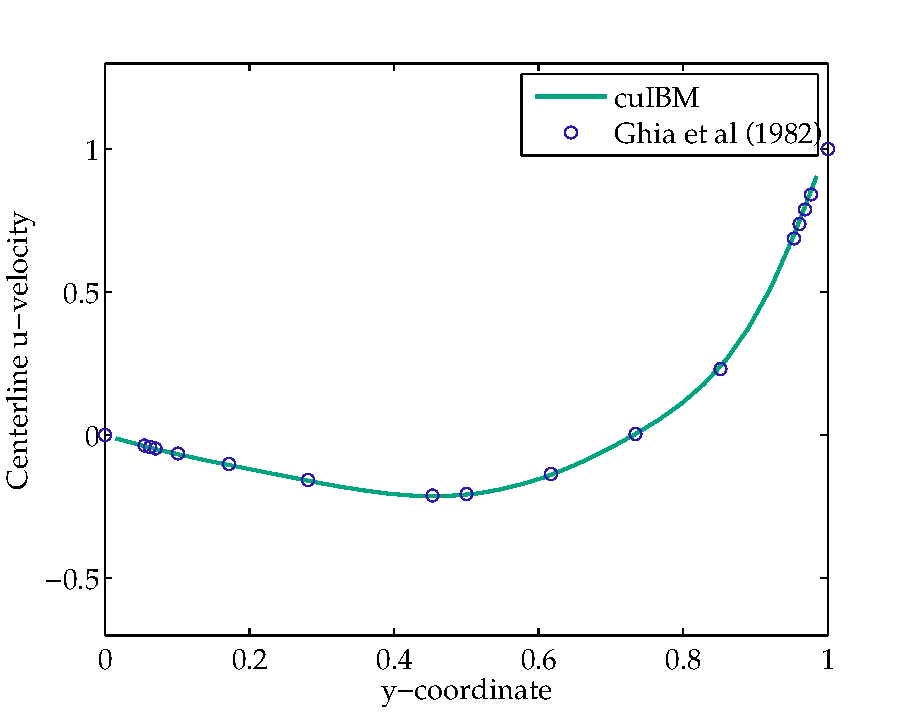
\includegraphics[width=0.45\linewidth]{cavRe100u.pdf}\label{fig:cavRe100a}}
	\subfloat[Velocity along the horizontal centerline,  $Re=100$.]
		{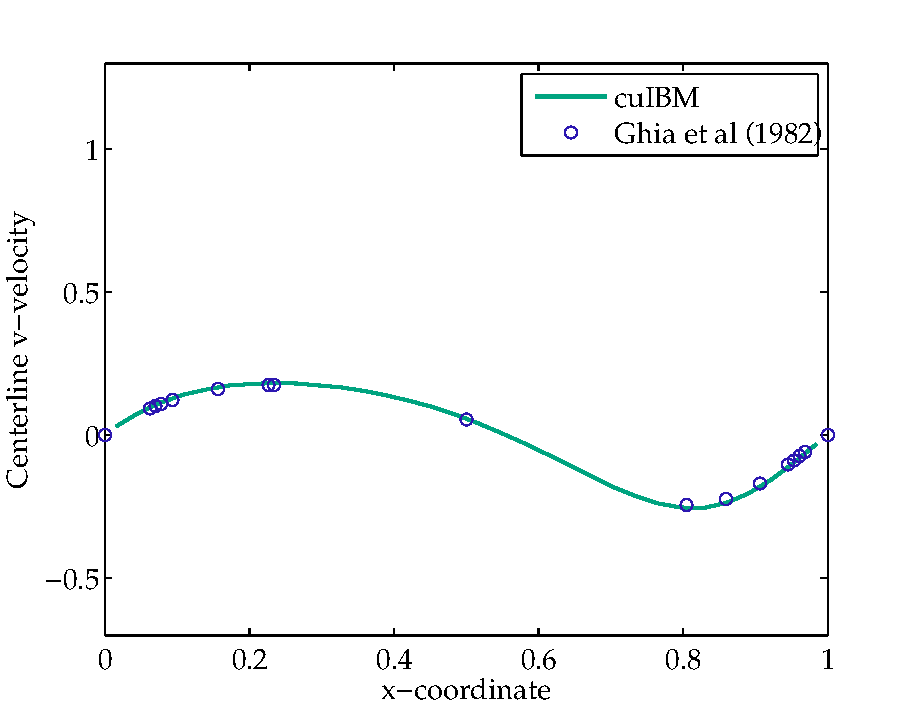
\includegraphics[width=0.45\linewidth]{cavRe100v.pdf}\label{fig:cavRe100b}}\\
	\subfloat[Velocity along the vertical centerline, $Re=1000$.]
		{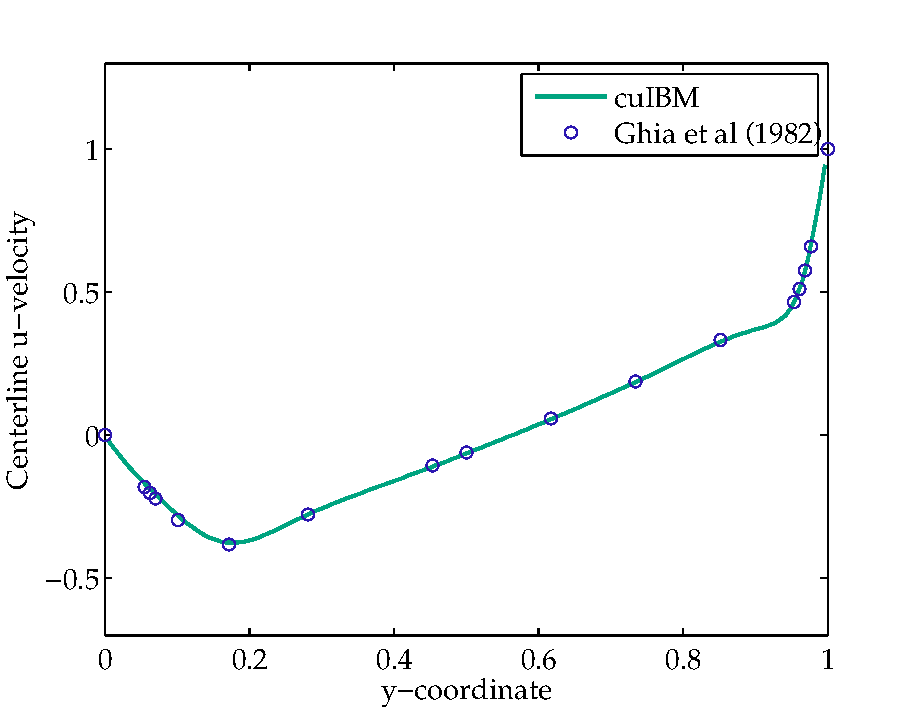
\includegraphics[width=0.45\linewidth]{cavRe1000u.pdf}\label{fig:cavRe1000a}}
	\subfloat[Velocity along the horizontal centerline,  $Re=1000$.]
		{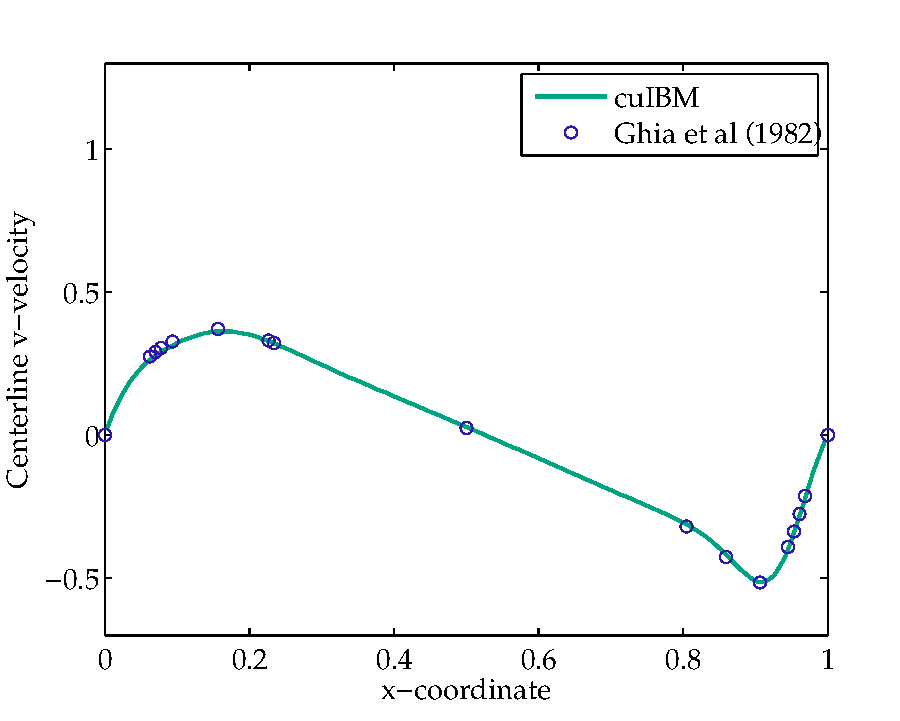
\includegraphics[width=0.45\textwidth]{cavRe1000v.pdf}\label{fig:cavRe1000b}}\vspace{0.4cm}\\
	\caption {Validation using a  lid-driven cavity.}
	\label{fig:cavity}
\end{figure*}


One of the simplest validation tests for a two-dimensional Navier-Stokes solver is the lid-driven cavity: the flow in a square cavity, with the top wall of the cavity (the lid) moving horizontally with constant velocity. This benchmark does not make use of the immersed boundary method but it is a test for the underlying Navier-Stokes solver. The Reynolds number is calculated using the speed of the lid, the length of the side of the square cavity and the kinematic viscosity of the fluid. The numerical solution was advanced in time until reaching steady state and the velocity is compared with the results by Ghia et al.\cite{GhiaETal1982} See Figure \ref{fig:cavity}. We used uniform grids, $32\times{32}$ for the $Re=100$ case and $128\times{128}$ for the the $Re=1000$ case. 




\subsection{Couette flow between concentric cylinders}

This is a simple validation test using an analytical solution, with the immersed boundary method in internal-flow mode. We calculate the flow between two concentric cylinders of radii $r_i=0.5$ and $r_o=1$, centered at the origin. The outer cylinder is held stationary while the inner cylinder is impulsively rotated from rest with an angular velocity  $\Omega=0.5$. The cylinders are contained in a square, stationary domain of side $1.5$, centered at the origin. 

The steady-state analytical solution for this flow is known. In the interior of the inner cylinder we have solid body rotation while between the two cylinders the azimuthal velocity is given by:
\begin{equation}
u_{\theta}(r)=\Omega\,{r_i}\frac{\left({r_o}/{r}-{r}/{r_o}\right)}{\left({r_o}/{r_i}-{r_i}/{r_o}\right)}.
\end{equation}

We set the kinematic viscosity to $\nu=0.03$ and obtained the numerical solution using six different grid sizes, ranging from $75\times{75}$ to $450\times{450}$, to calculate the observed order of convergence. Figure \ref{fig:couette}\subref{fig:spatial} shows plots of the $L^2$ and $L^\infty$ norms of the relative errors, verifying that the scheme provides first-order accuracy in space, as expected for the \ibm\ formulation we used.


\begin{figure*}
	\subfloat[Comparison of the numerical and analytical solutions.]{
		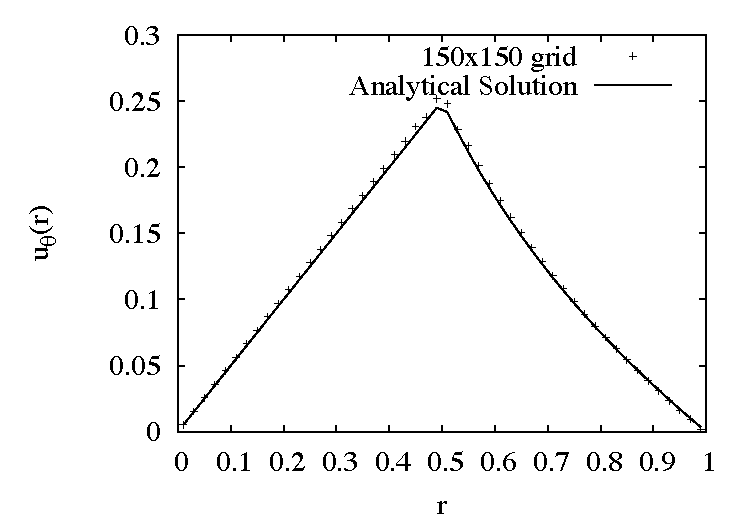
\includegraphics[width=0.45\linewidth]{validate.pdf}\label{fig:validate}}
	\subfloat[Convergence, showing errors for different grid sizes.]{
		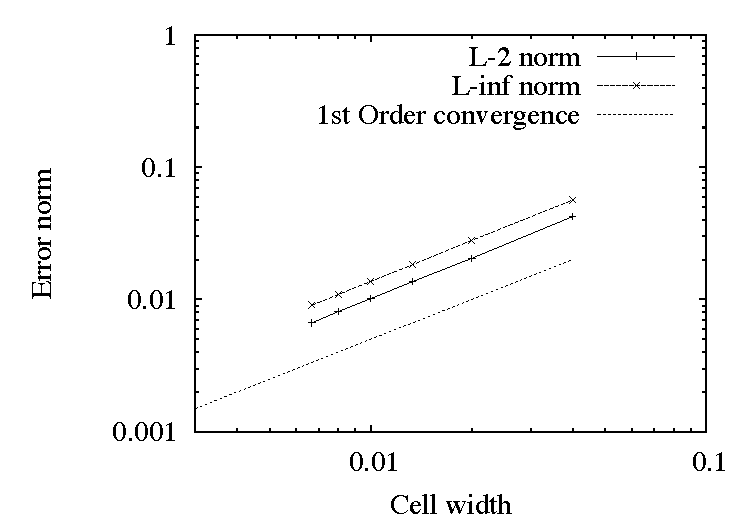
\includegraphics[width=0.45\linewidth]{spatial.pdf}\label{fig:spatial}}\vspace{0.4cm}\\
	\caption{Validation using the Couette flow problem.}
	\label{fig:couette}
\end{figure*}

To verify the temporal order of convergence, we ran a simulation from $t=0$ to $t=8$ on a $151\times 151$ grid, using different time steps ($\Delta{t}=0.01,~0.005~\text{and}~0.0025$). Both first- and third-order accurate expansions of $B^N$ were used and the calculated orders of convergence (using the $L^2$ norms of the differences in the solutions) at various times have been summarised in Table \ref{table:temporal}, and are as expected.

\begin{table}[h]
  \centering
  \fontfamily{ppl}\selectfont
    \begin{tabular}{ c c c }
 \toprule
     & Order of convergence & Order of convergence \\
    Time & ($N=1$) & ($N=3$) \\ 
    \midrule
    0.8 & 0.97 & 2.67 \\ 
    2 & 0.99 & 2.85 \\ 
    4 & 0.93 & 2.73 \\ 
    8 & 0.97 & 2.83 \\ 
    \bottomrule
    \end{tabular}
    \caption{Observed temporal order of convergence at different times for Couette-flow test.}\vspace{0.25cm}
    \label{table:temporal}
\end{table}


\subsection{Flow over an impulsively started cylinder}

We performed a convergence test for the flow over an impulsively started cylinder at Reynolds number $40$. We also obtained numerical solutions of the flow over an impulsively started circular cylinder at Reynolds numbers $40$, $550$ and $3000$, looking at the vorticity contours and comparing the drag coefficient with experimental values published in the literature\cite{Tritton1959} and with past computations.\cite{Koumoutsakos1995}  
The cylinder has diameter $d=1$, is centered at the origin and is placed in an external flow with free-stream velocity $u_{\infty}=1$. The initial velocity is uniform throughout the domain, a square centered at the origin with sides of length $30$. The fluid flows from left to right, and the velocity on the left, top and bottom edges was set to the free-stream velocity. A convective boundary condition (${\partial{u}}/{\partial{t}}+u_{\infty}{\partial{u}}/{\partial{x}}=0$) was used on the right edge of the domain.

For the spatial convergence test, the flow at Reynolds number $40$ was simulated using four uniform grids of size $400\times 400$, $600\times 600$, $900\times 900$ and $1350\times 1350$ in the specified domain. The simulations were run for a length of non-dimensional time $30$, and the $x$-velocity field at the end of each of these runs was computed on a uniform grid of size $41\times 41$ in the region $[-1,1]\times[-1,1]$ using bilinear interpolation. The $L2$-norm of the difference between values on this grid from solutions on two consecutive grids is plotted against the bigger of the mesh sizes in Figure \ref{cylRe40convergence}. For example, the $y$-coordinate of the first point on the graph is the $L2$-norm of the difference in the $x$-velocities on the $41\times 41$ grid for the two cases using the $400\times 400$ grid and the $600\times 600$ grid, and the $x$-coordinate of the point is 600. This $x$-coordinate is proportional to the inverse of the cell width because the grid used is uniform. These grids are chosen such that the ratio of the cell widths of consecutive grids is a constant, which in this case is $1.5$. The slope of the graph in Figure \ref{cylRe40convergence} gives the order of convergence of the method \cite{Roache1998}. The linear least squares fit through the three points gives us an order of convergence of $1.03$, as expected.

\begin{figure}
\centering
	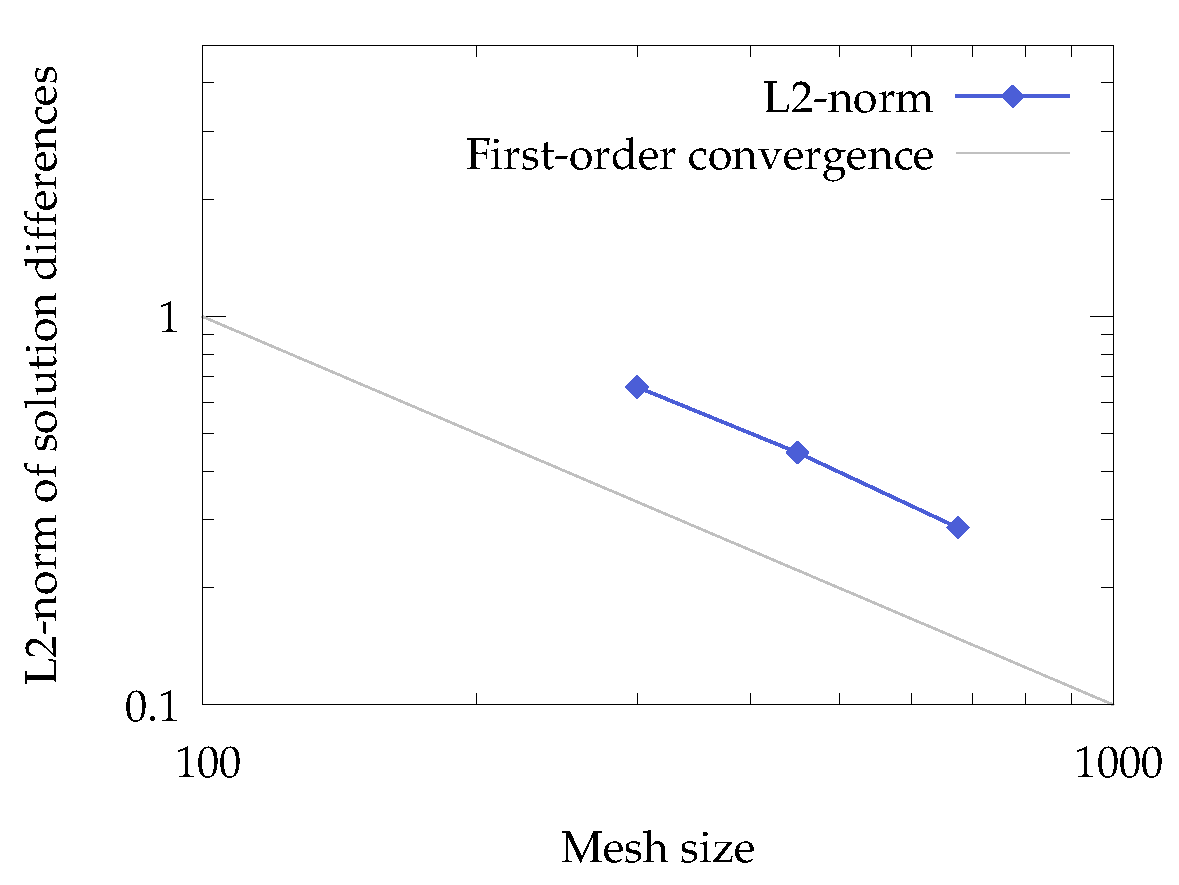
\includegraphics[width=0.75\textwidth]{figs/cylRe40Convergence.pdf}
	\caption{Convergence plot for flow over a circular cylinder at Reynolds number $40$. The $L2$-norms of the difference between successive solutions obtained on four different grids (whose cell widths are separated by a constant ratio) are plotted on the graph against the grid size.}
	\label{cylRe40convergence}
\end{figure}

The flow computations at Reynolds numbers $40$, $550$ and $3000$ which were performed for validation used grids that had minimum cell widths of $0.02$, $0.01$ and $0.004$ respectively near the solid boundaries. The grid is uniform in a small rectangular region encompassing the body, and is stretched exponentially beyond this region till the edges of the domain. See Table \ref{table:gridinfo} for all grid details.
	

\begin{figure*}[h]
	\subfloat[Steady state vorticity field.]
		{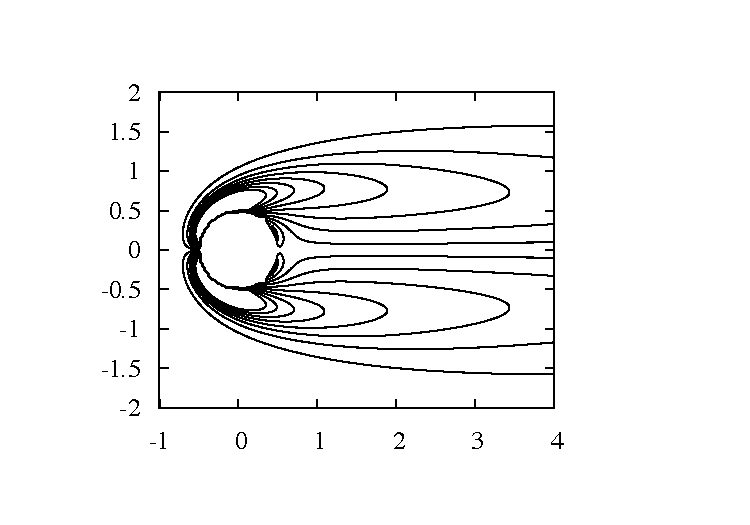
\includegraphics[width=0.34\textwidth]{figs/vortRe40.pdf}}
	\subfloat[Time-varying drag coefficient.]
		{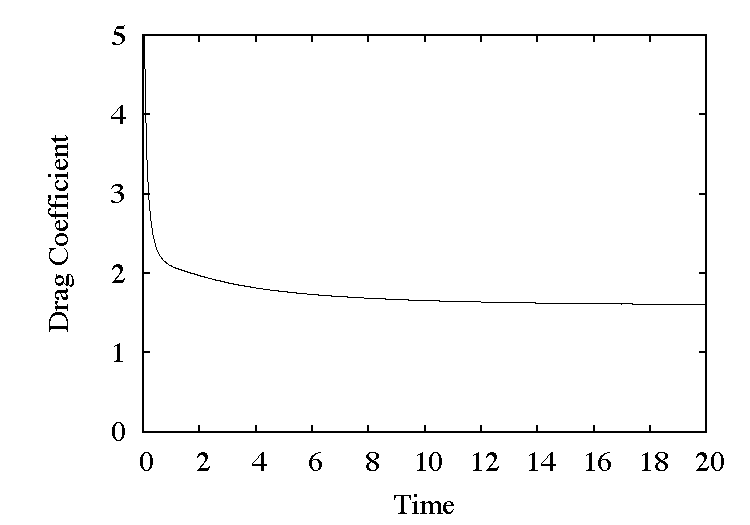
\includegraphics[width=0.4\textwidth]{figs/dragRe40.pdf}}\vspace{0.4cm}\\
\caption {Validation with external flow over a circular cylinder at $Re=40$. Contour lines in (a) are drawn from $-3$ to $3$ in steps of $0.4$.}
	\label{fig:Re40}
\end{figure*}



The flow at $Re=40$ reaches a steady state with a drag coefficient of $1.57$, which matches the experimental value. The vorticity fields and the unsteady drag coefficients for the cases with $Re=550$ and $3000$ also agree well with past computations of Koumoutsakos and collaborators. The results are presented in Figures \ref{fig:Re40}--\ref{fig:Re3000}.


\begin{table}[t]
  \centering
  \fontfamily{ppl}\selectfont
    \begin{tabular}{ c c c c c}
	\toprule
	Re & $n_x \times n_y$ & $\Delta{x}_{min}$ & Extent of uniform grid & $r_{stretching}$\\
	\midrule
	$40$ & $330 \times 330$ & $0.02$ & $[-0.54,0.54]$ & $1.02$\\	
	$550$ & $450 \times 450$ & $0.01$ & $[-0.54,0.54]$ & $1.02$\\	
	$3000$ & $986 \times 986$ & $0.004$ & $[-0.52,0.52]$ & $1.01$\\
	\bottomrule
    \end{tabular}
    \caption{Grid information for the impulsively started cylinder tests.}\vspace{0.25cm}
    \label{table:gridinfo}
\end{table}

\begin{figure*}[t]		
	\subfloat[Vorticity field at non-dimensional time $3.0$]
		{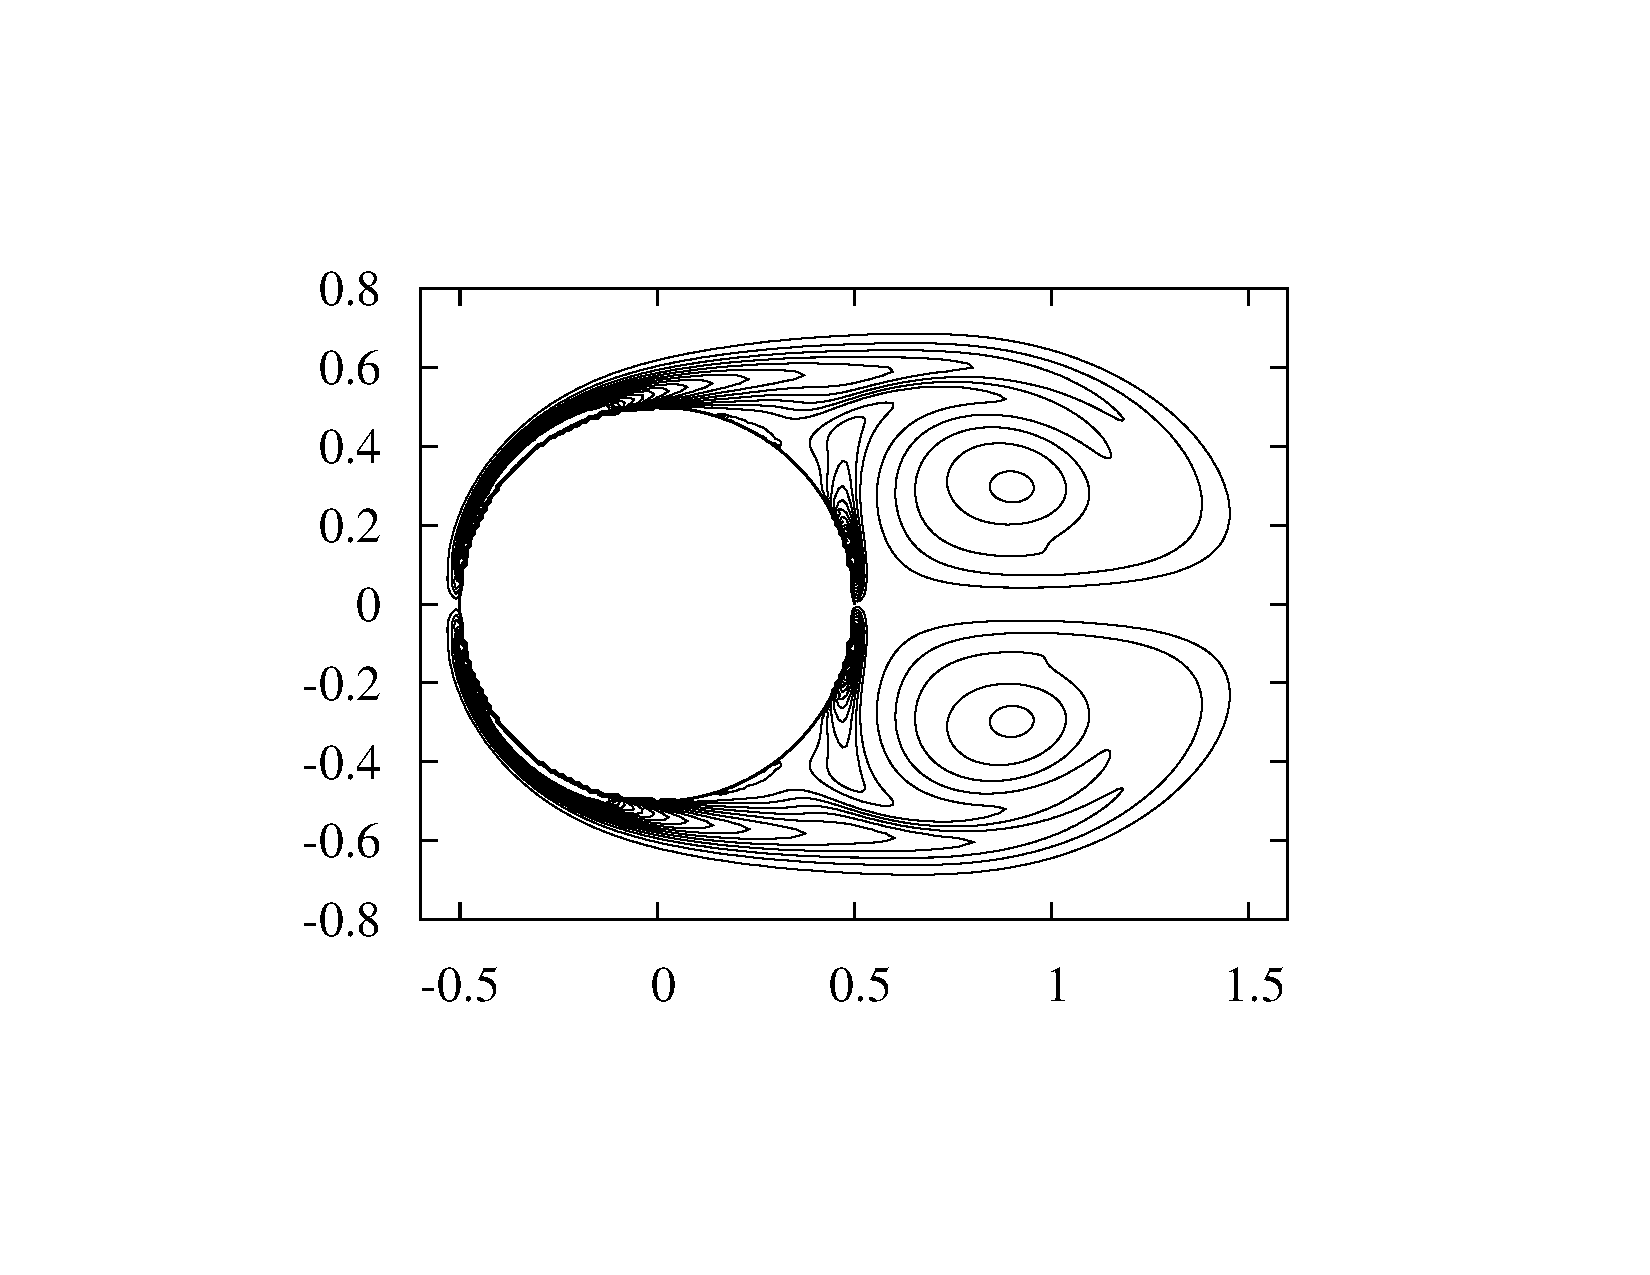
\includegraphics[width=0.36\textwidth]{figs/vortRe550.pdf}} \quad
	\subfloat[Time-varying drag coefficient.]
		{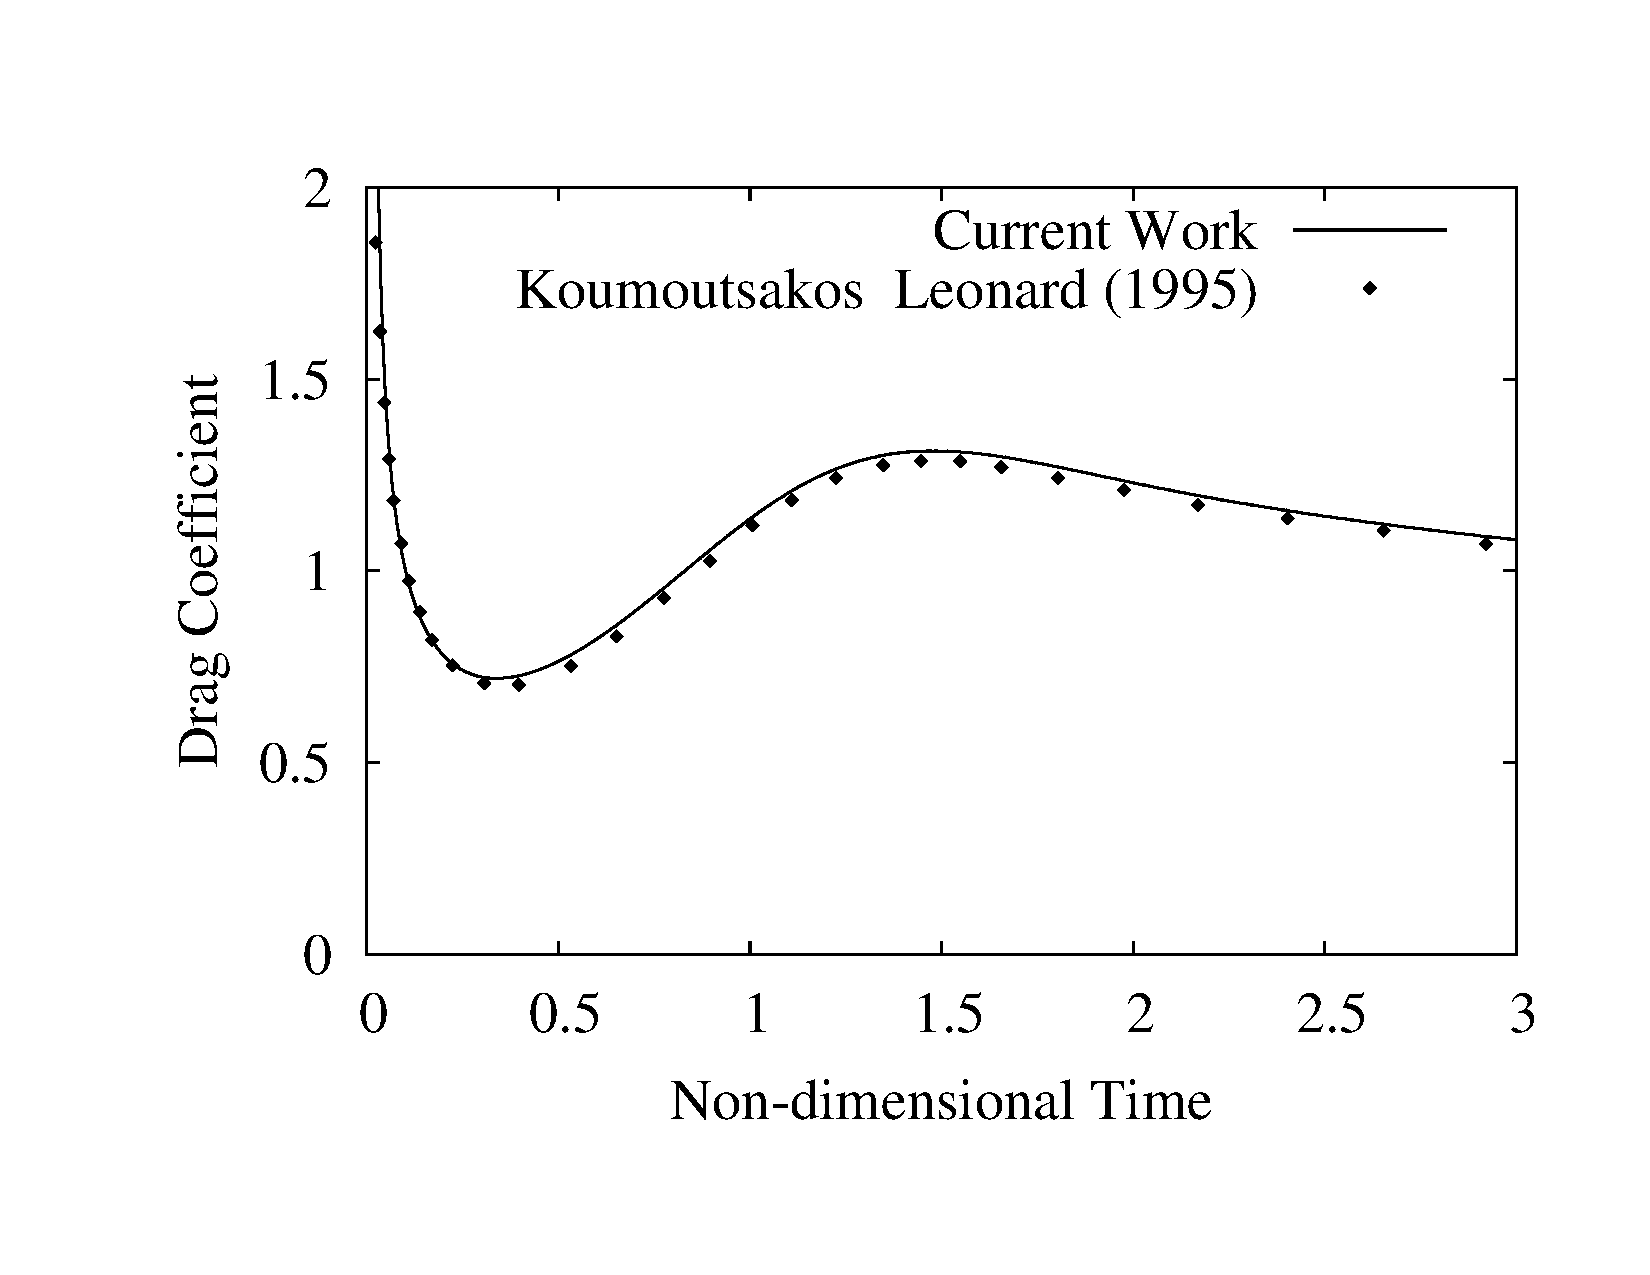
\includegraphics[width=0.4\textwidth]{figs/dragRe550.pdf}}
	\label{fig:Re550}
%\end{figure*}	
%	
%\begin{figure*}%[htb]	
	\subfloat[Vorticity field at non-dimensional time $3.0$]
		{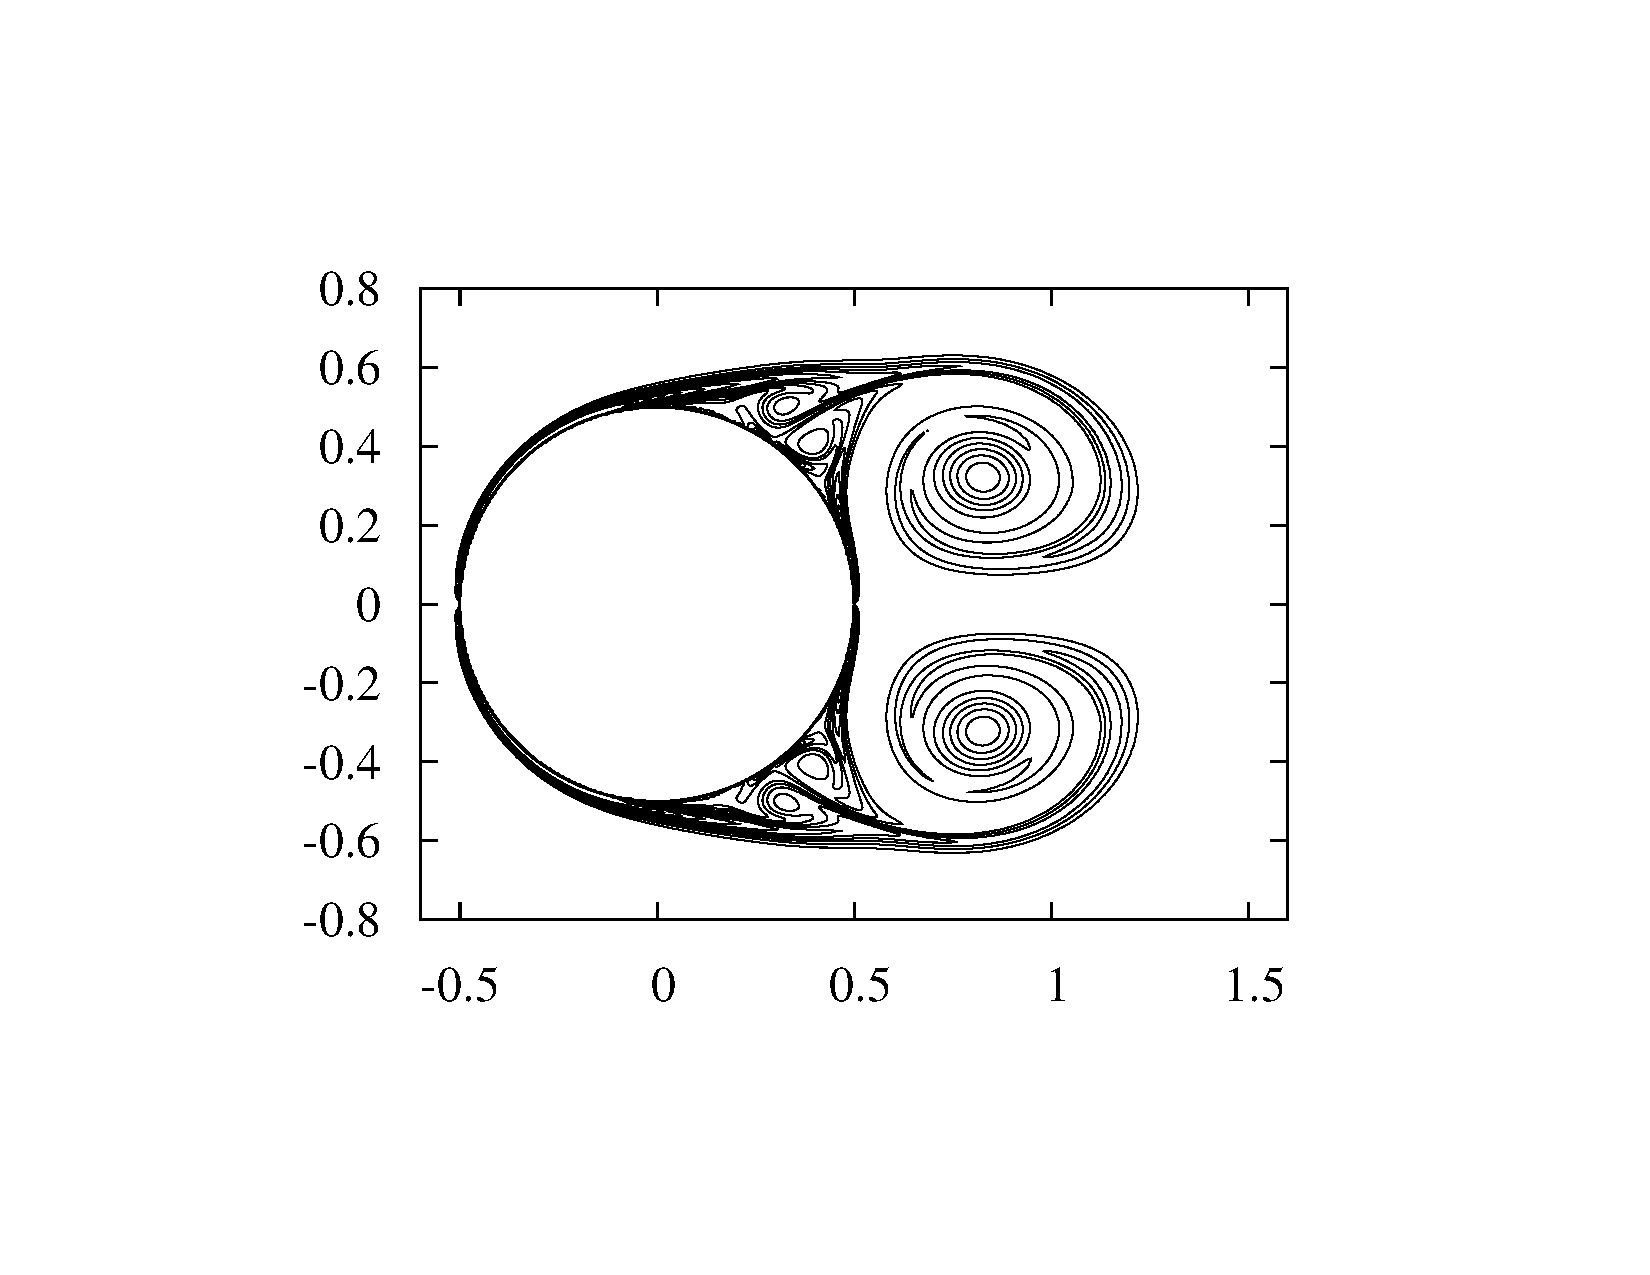
\includegraphics[width=0.37\textwidth]{figs/vortRe3000.pdf}} \quad
	\subfloat[Time-varying drag coefficient.]
		{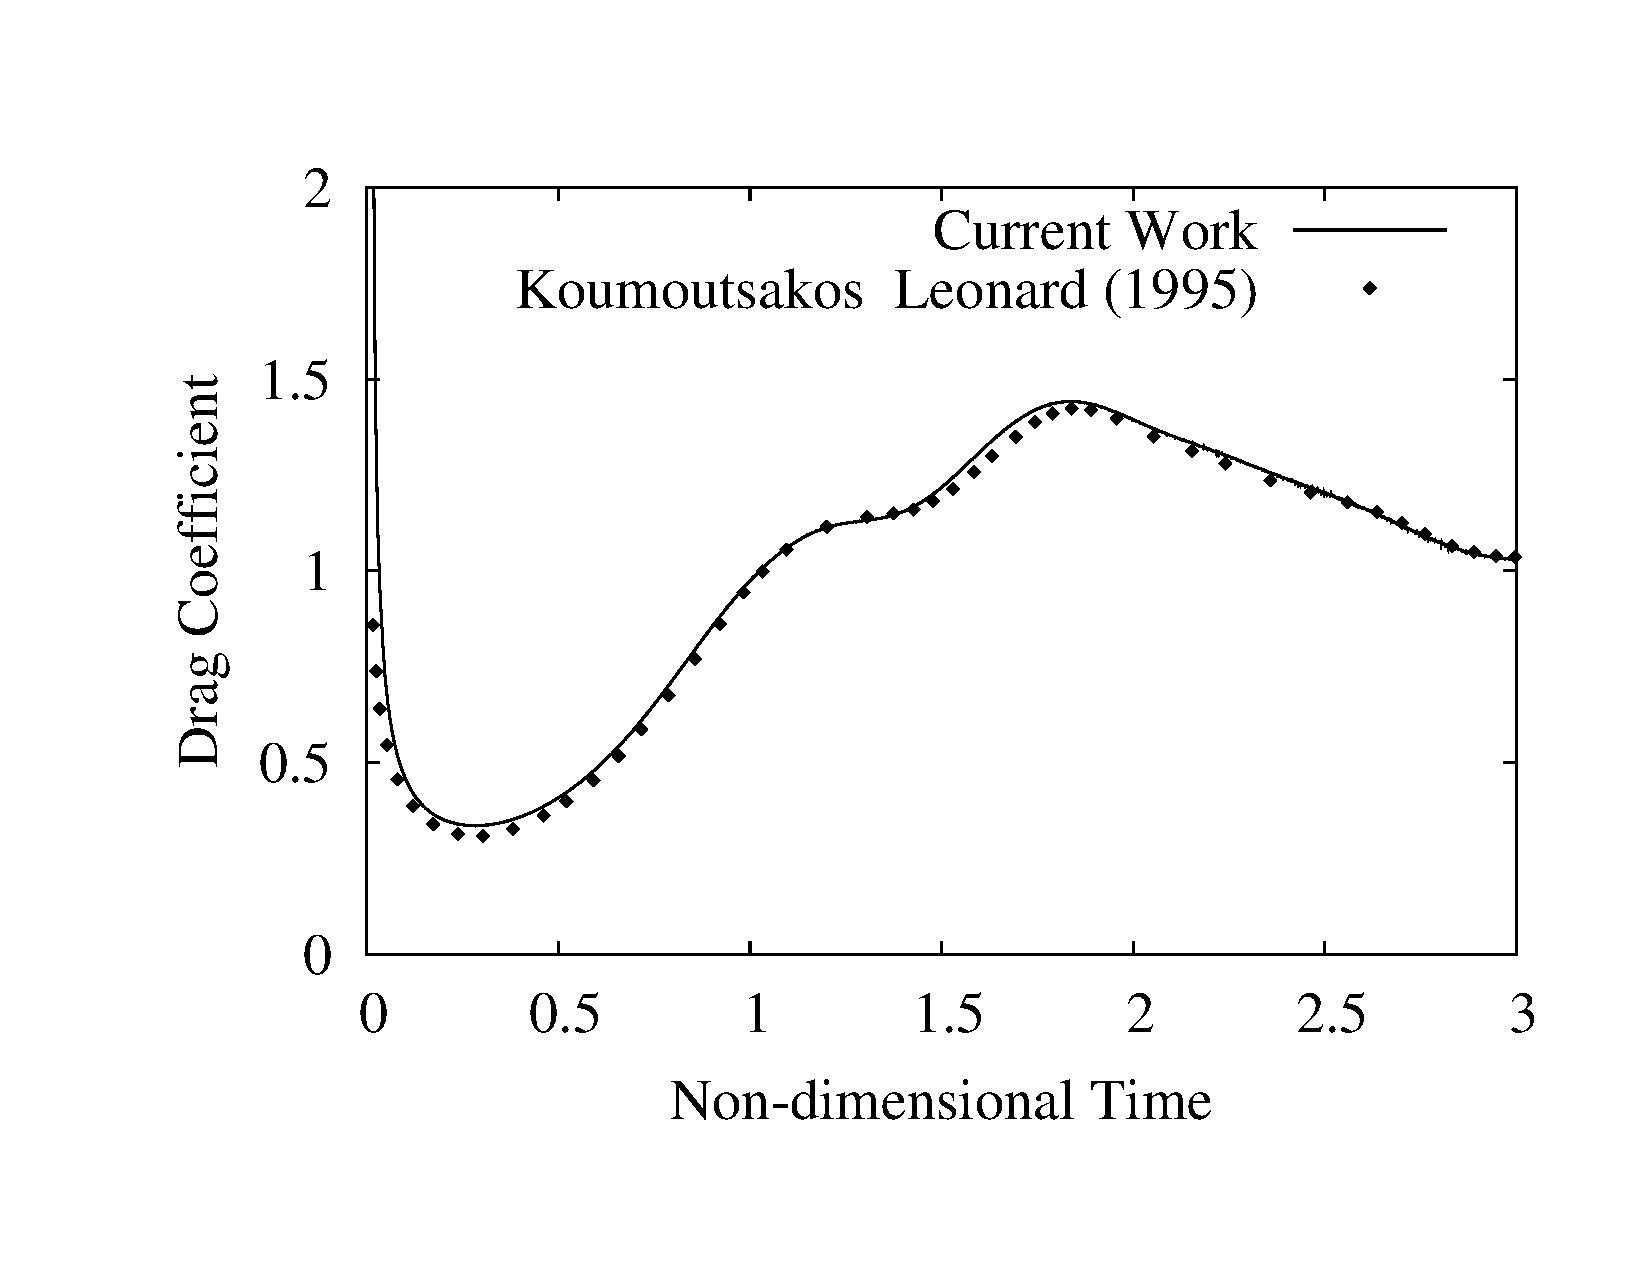
\includegraphics[width=0.4\textwidth]{figs/dragRe3000.pdf}}\vspace{0.4cm}\\
\caption{Validation with impulsively started flow over a circular cylinder at Reynolds 550 (top) and 3000 (bottom). The contour lines in (a) are drawn from $-32$ to $32$ in steps of $2$, and in (c) from $-56$ to $56$ in steps of $4$, both excluding the zero contour.}
	\label{fig:Re3000}
\end{figure*}

\subsection{Flow over a NACA 0008 airfoil}

We simulated Reynolds number 2000 flow over a NACA 0008 airfoil at an angle of attack of $4^\circ$, and computed the steady state lift and drag coefficients. We performed these calculations for two different mesh sizes, with minimum cell widths $0.004$ and $0.002$ near the body. The grids are generated in a way similar to the cylinder cases in the previous section, but with the uniform grid near the body encompassing the area $[-0.6,0.6]\times[-0.1,0.1]$ and the stretching ratio fixed at $1.007$. The flow was impulsively started, and the force coefficients at the instant of non-dimensional time $t^*=12$ were noted as the steady state values. The results are summarised in Table \ref{table:naca0008}. For the case when then minimum cell width is $0.002$, we see a difference in lift coefficient of less than 1\% and a difference of about 4\% in drag coefficient when compared to a previous study by Kunz and Kroo.\cite{Kunz2000}

\begin{table}[t]
  \centering
  \fontfamily{ppl}\selectfont
    \begin{tabular}{ c c c c c }
	\toprule
	Case & $C_l$ & $\Delta{C_l}/C_l$ & $C_d$ & $\Delta{C_d}/C_d$\\
	\midrule
	Kunz \& Kroo (2000) & 0.0805 & & 0.272 & \\	
	$h=0.004$ & 0.0819 & 1.7\% & 0.2834 & 4.2\% \\	
	$h=0.002$ & 0.0810 & 0.6\% & 0.283 & 4.0\% \\
	\bottomrule
    \end{tabular}
    \caption{Lift and drag coefficients of a NACA 0008 airfoil at angle of attack $4^\circ$ in $Re=2000$ flow.}\vspace{0.25cm}
    \label{table:naca0008}
\end{table}

\subsection{Unsteady flow over a circular cylinder}

We obtained longer runs of flow around a circular cylinder, resulting in a von K{\'a}rm{\'a}n vortex street. 
The cylinder of diameter $1$ is placed at the center of a domain of size $30\times 30$, its initial position slightly offset in the $y$-direction and then brought to the center at the beginning of the run to trigger the instability in the flow and cause vortex shedding. The minimum cell width in the grids was $0.02$, maintained in the wake region behind the cylinder. To the left, top and bottom of the cylinder, the grid stretches with an exponential ratio of $1.02$. 
Table \ref{table:wakeresults} lists the results obtained at different Reynolds numbers, comparing the Strouhal number of the vortex shedding with the experimental results of Williamson.\cite{Williamson1996}


\begin{table}%[h]
\  \centering
  \fontfamily{ppl}\selectfont
	\begin{tabular} {c c c c c}
		\toprule
		$Re$ & $C_l$ & $C_d$ & $St$ & $St_{\text{exp}}$ \\
		\midrule
		$100$ & $\pm{0.339}$ & $1.37\pm{0.009}$ & $0.166$ & $0.164$\\
		
		$150$ & $\pm{0.532}$ & $1.35\pm{0.026}$ & $0.185$ & $0.184$\\
		
		$200$ & $\pm{0.688}$ & $1.36\pm{0.042}$ & $0.197$ & $0.197$\\
		\bottomrule
	\end{tabular}
	\caption{Computed data for flow past a circular cylinder at different Reynolds numbers and comparison with experimental results.}\vspace{0.3cm}
	\label{table:wakeresults}
\end{table}


\begin{figure}
\centering
	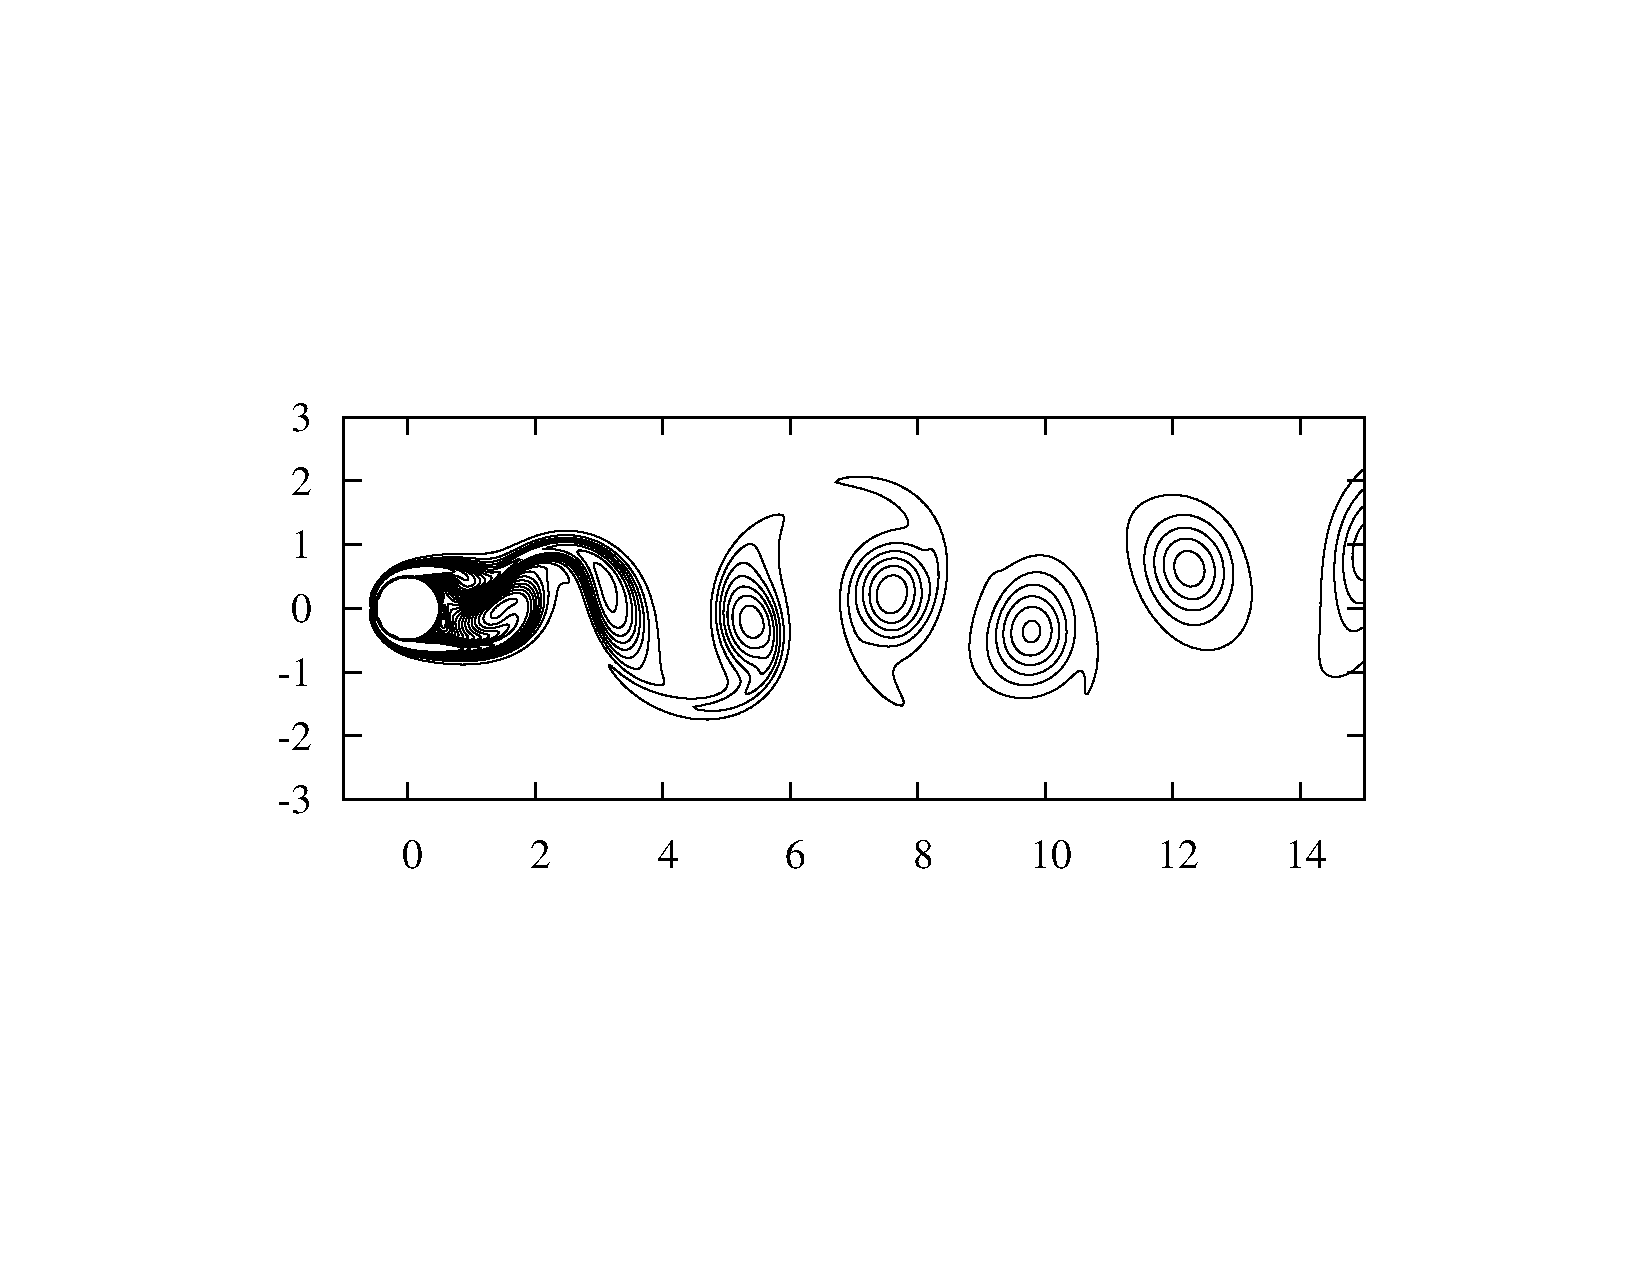
\includegraphics[width=0.85\textwidth]{figs/wakeRe200.pdf}
	\caption{Flow over a circular cylinder at Reynolds number $200$. Vorticity contours from $-5$ to $5$ in increments of $0.4$.}
\end{figure}


\newthought{The results above} validate our code with both analytical results and experimental benchmarks for flows with stationary solid interfaces. The following cases demonstrate the capability of the code to reproduce past results for flows with moving boundaries. The first case is the heaving airfoil in a uniform flow computed by Lewin and Haj-Hariri\cite{Lewin2003} and the second case is an airfoil that performs both pitching and heaving motions, simulating the flapping motion of an insect wing, as computed by Wang et al.\cite{WangETal2004}


\subsection{\large Unsteady flow of a heaving airfoil}

We computed the flow of an elliptic airfoil of thickness-to-chord ratio $0.12$ and chord length $c=1$ submerged in a   free stream with velocity $u_\infty=1.0$. The airfoil oscillates in the direction perpendicular to the free-stream velocity with frequency $f$ and amplitude $Y_{max}$. 
The problem parameters are the reduced frequency $k={2{\pi}{f}{c}}/{u_\infty}=2$, the non-dimensional maximum heaving velocity $kh={k}{Y_{max}}/{c}=0.8$, and the Reynolds number, $Re={u_\infty}c/{\nu}=500$. The domain size is $30 \times30$ and the near-body region in $[-0.52,0.52]\times[-0.52,0.52]$ has a uniform grid of width $0.005$, and exponentially stretched grids apply in front of the airfoil (stretching ratio of $1.02$), in the $y$-direction above and below the body (stretching ratio $1.015$), and in the region $[0.52,0.78]$ immediately behind the airfoil (stretching ratio $1.02$); a uniform grid of size $0.01$ follows from that region to the edge of the domain. The total size of the mesh is $1339\times{686}$ and the time step used was $0.0005$. The boundary conditions are the same as those used for the earlier cases of external flow over a cylinder. The vorticity field as shown in Figure \ref{fig:heaving} matches the results in Fig.~3 of Lewin and Haj-Hariri.

\begin{figure*}
	\subfloat[$t^*=7.125$]{ 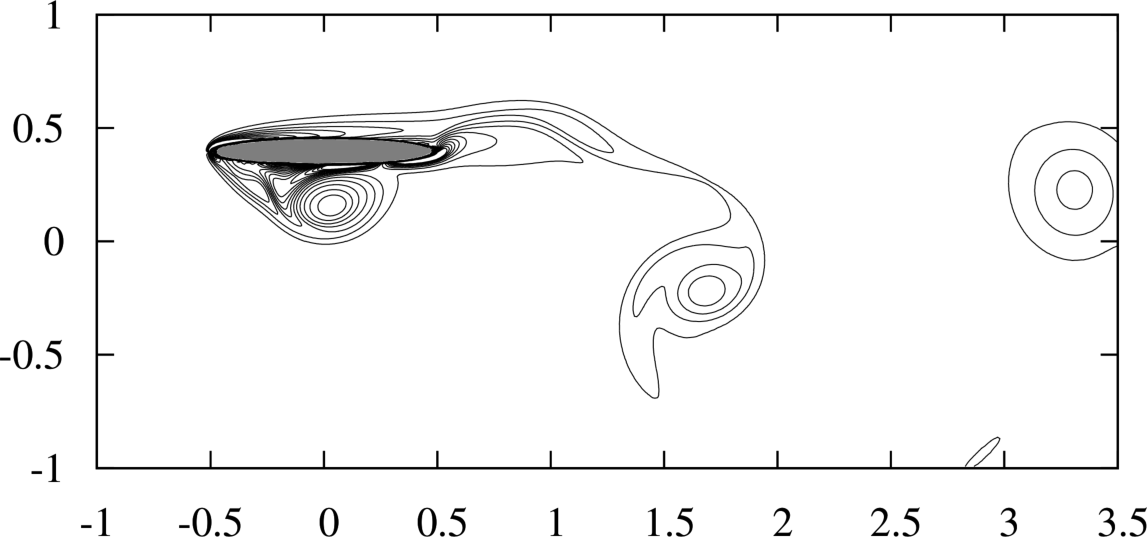
\includegraphics[width=0.48\textwidth]{h500a.pdf} }
	\subfloat[$t^*=7.3125$]{ 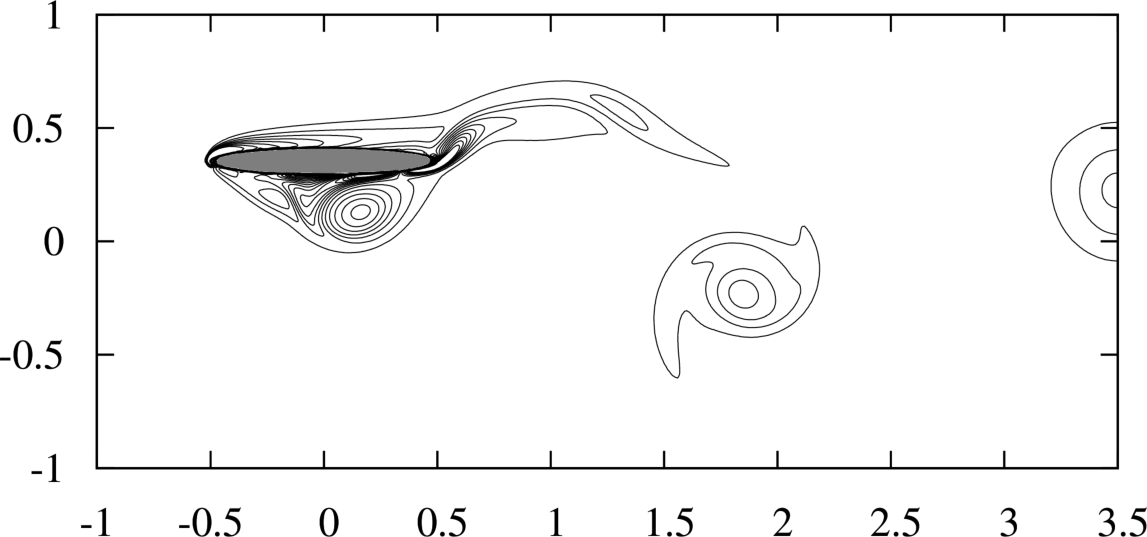
\includegraphics[width=0.48\textwidth]{h500b.pdf} } \\
	\subfloat[$t^*=7.5$]{ 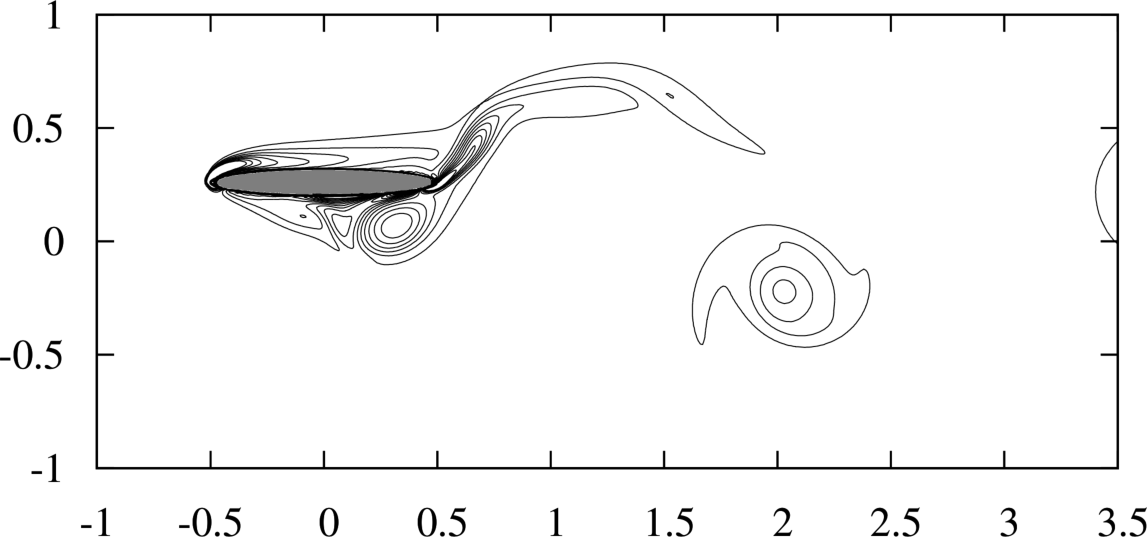
\includegraphics[width=0.48\textwidth]{h500c.pdf} }
	\subfloat[$t^*=7.6875$]{ 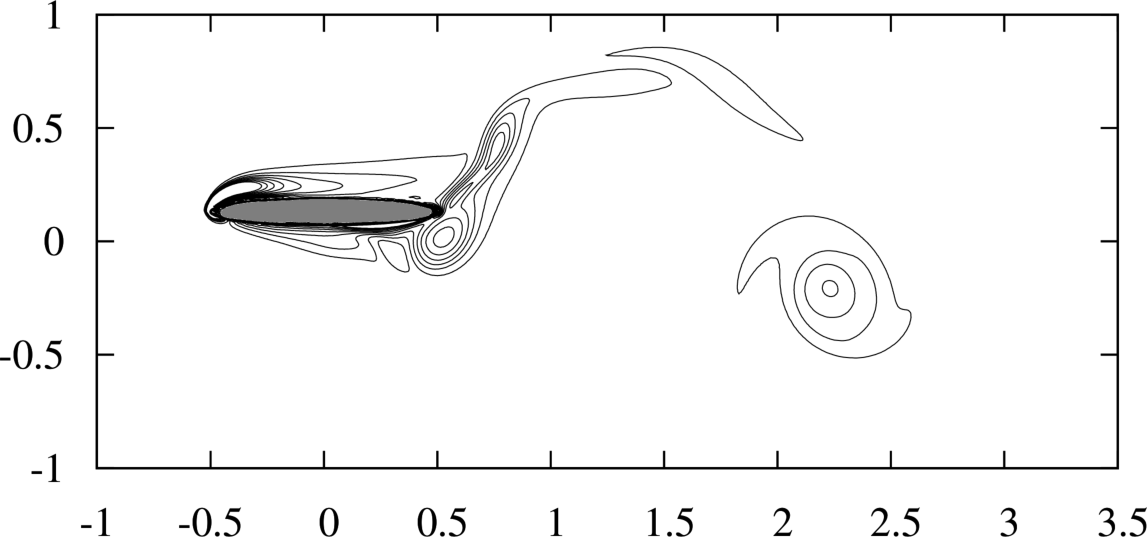
\includegraphics[width=0.48\textwidth]{h500d.pdf} } \\
	\subfloat[$t^*=8.0625$]{ 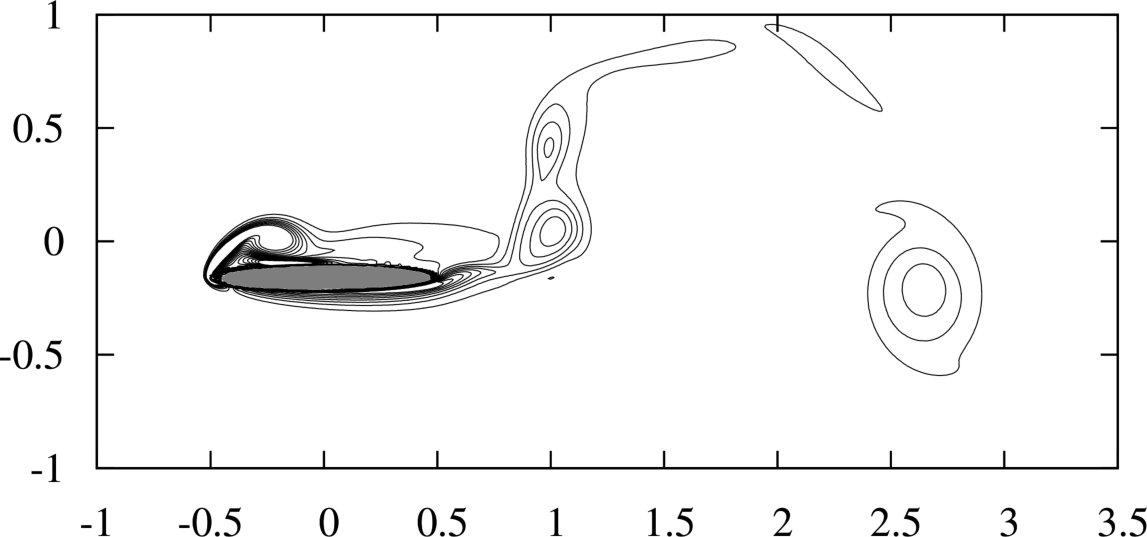
\includegraphics[width=0.48\textwidth]{h500e.pdf} }
	\subfloat[$t^*=8.4375$]{ 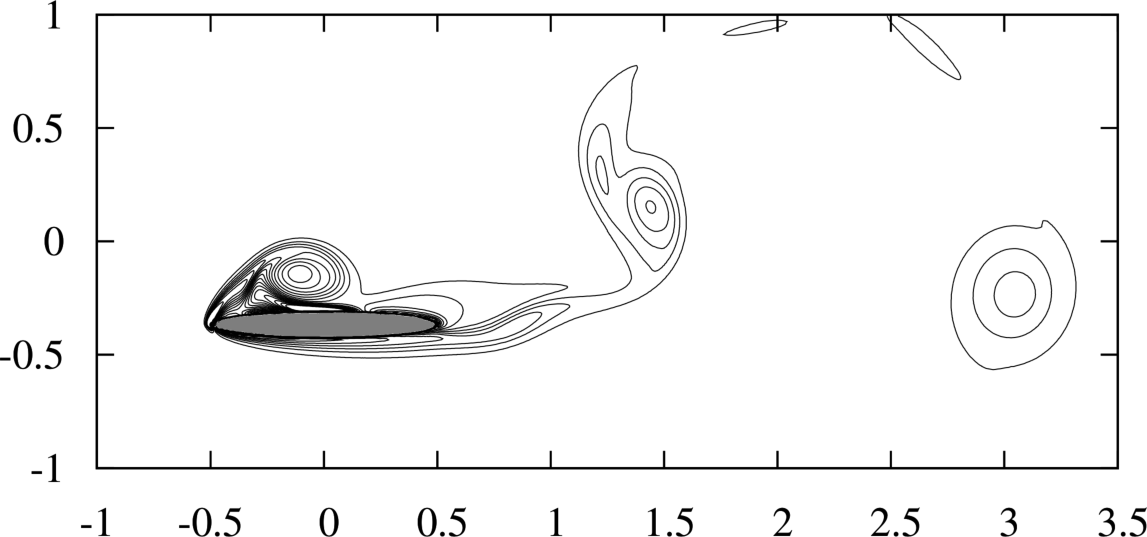
\includegraphics[width=0.48\textwidth]{h500f.pdf} }
\caption{Vorticity field for the downstroke of the heaving airfoil, with contours drawn at levels $\pm{2}$, $\pm{6}$, $\pm{10}$, etc.}\vspace{0.4cm}\\
\label{fig:heaving}
\end{figure*}


\subsection{\large Flow due to a flapping airfoil}

We consider a flapping airfoil, the motion of which is described by
\begin{align}
	x(t) = \frac{A_0}{2} \cos (2{\pi}{f}{t}) \nonumber \\
	\alpha (t) = \alpha_0 + \beta \sin ( 2{\pi}{f}{t} + \phi ), \nonumber
\end{align}
where $x(t)$ is the position of the center of the airfoil and $\alpha(t)$ is the angle made by the airfoil with the line of oscillation. The airfoil is elliptical with a thickness-to-chord ratio of $0.12$ and rotates about its center. The Reynolds number is calculated using the maximum translational velocity of the airfoil and the chord length. We consider the case with symmetrical rotation $(\phi=0)$ at Reynolds number $75$ and with ${A_0}/{c}=2.8$, $\alpha=\pi/2$, $\beta=\pi/4$ and $f=0.25$ Hz.

The airfoil has chord length $1$ and oscillates at the center of a domain, each side of which is $30$ chord-lengths long. The grid is uniform in the region $[-2,2]\times[-0.52,0.52]$ with cell width $0.01$ and beyond this region it is stretched with a ratio of $1.01$ on all sides, resulting in a mesh size of $930\times{654}$ cells. The time step used is $0.001$.

The vorticity field at different times during the first cycle is shown in Figure \ref{fig:flapping} and a comparison of the unsteady lift coefficient with the computational and experimental results presented by Wang et al.\ is plotted in Figure \ref{fig:flapCl}. The experiments were conducted with a three-dimensional wing and both simulations were performed in two dimensions, hence we don't expect them to exactly match. But we note that the computational results follow the expected trend and agree reasonably well with the experimental results.

\begin{figure}
\centering
    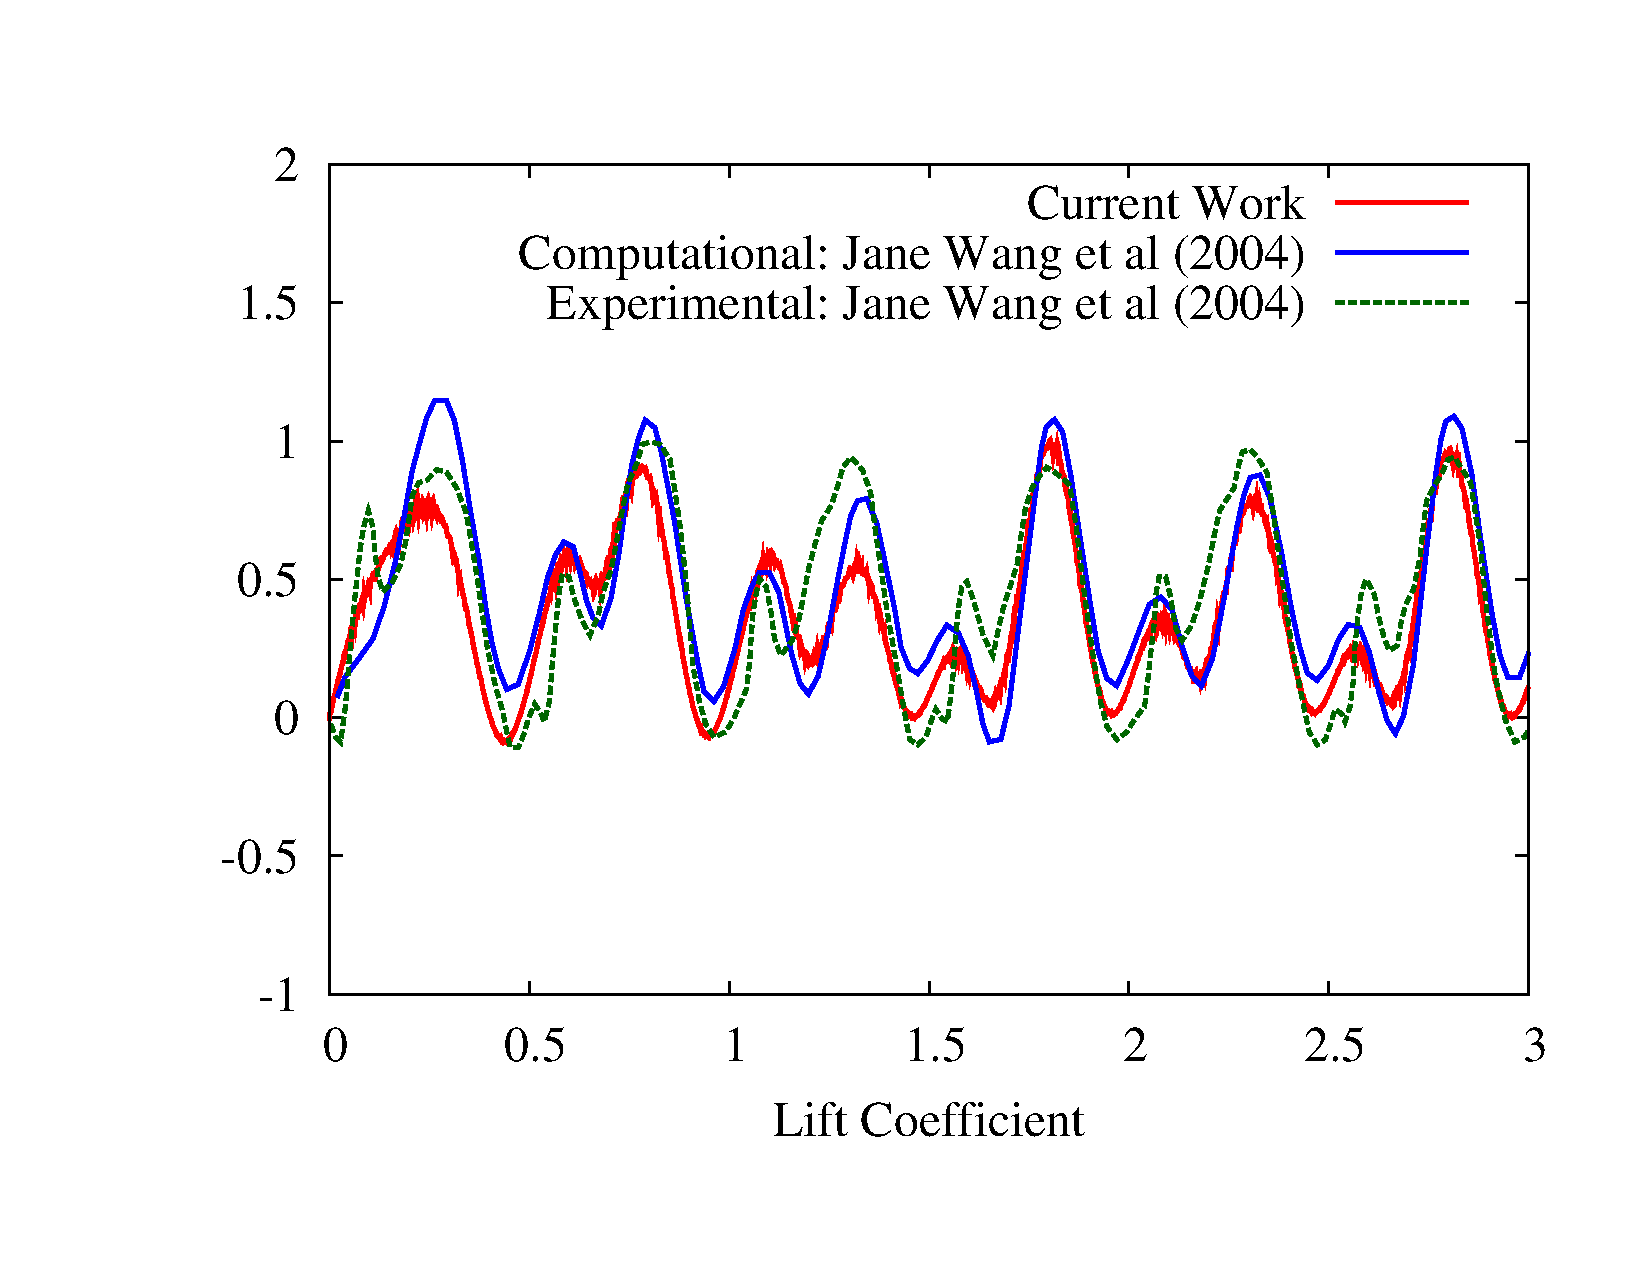
\includegraphics[width=0.75\linewidth]{flapCl.pdf}
    \caption{Unsteady lift coefficient for the first three cycles of a flapping airfoil. Time is non-dimensionalized with the  period of oscillation and the lift coefficient is calculated by normalizing the lift force with respect to the maximum of the quasi-steady force experienced by the airfoil.}
    \label{fig:flapCl}
\end{figure}

\begin{figure*}
$\begin{array}{cc}
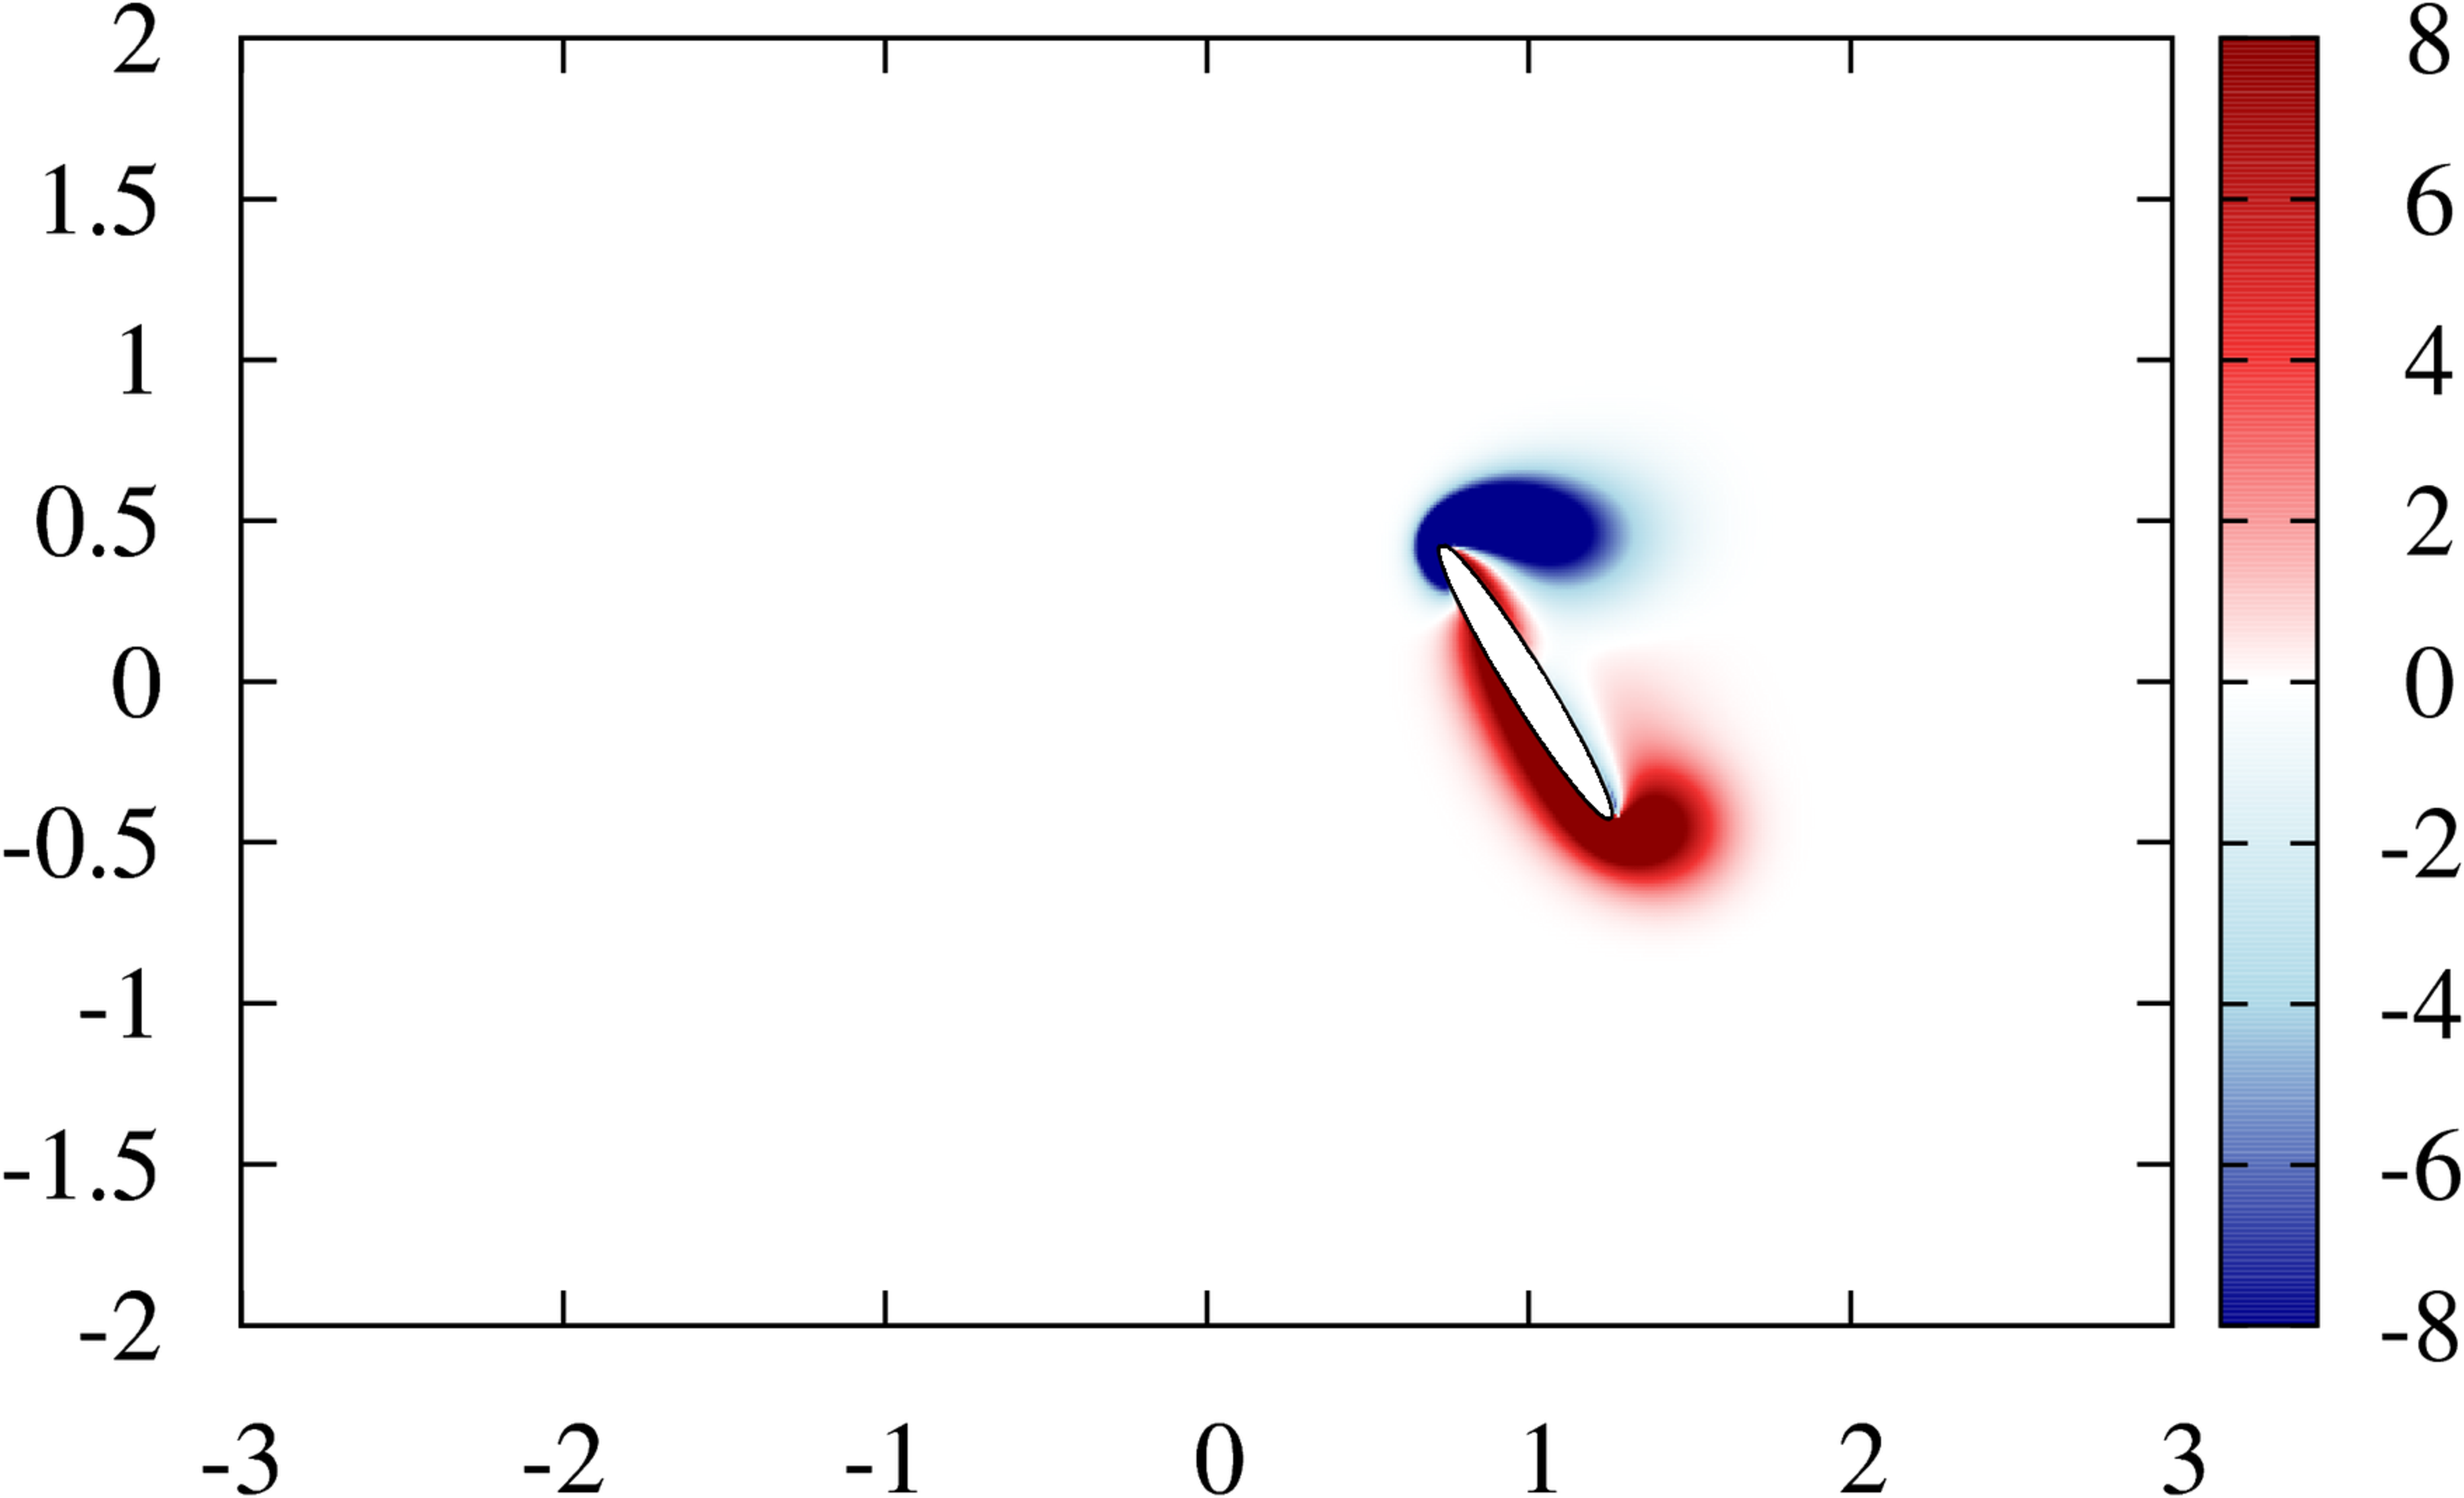
\includegraphics[width=0.4\textwidth]{figs/flap0500.pdf} &
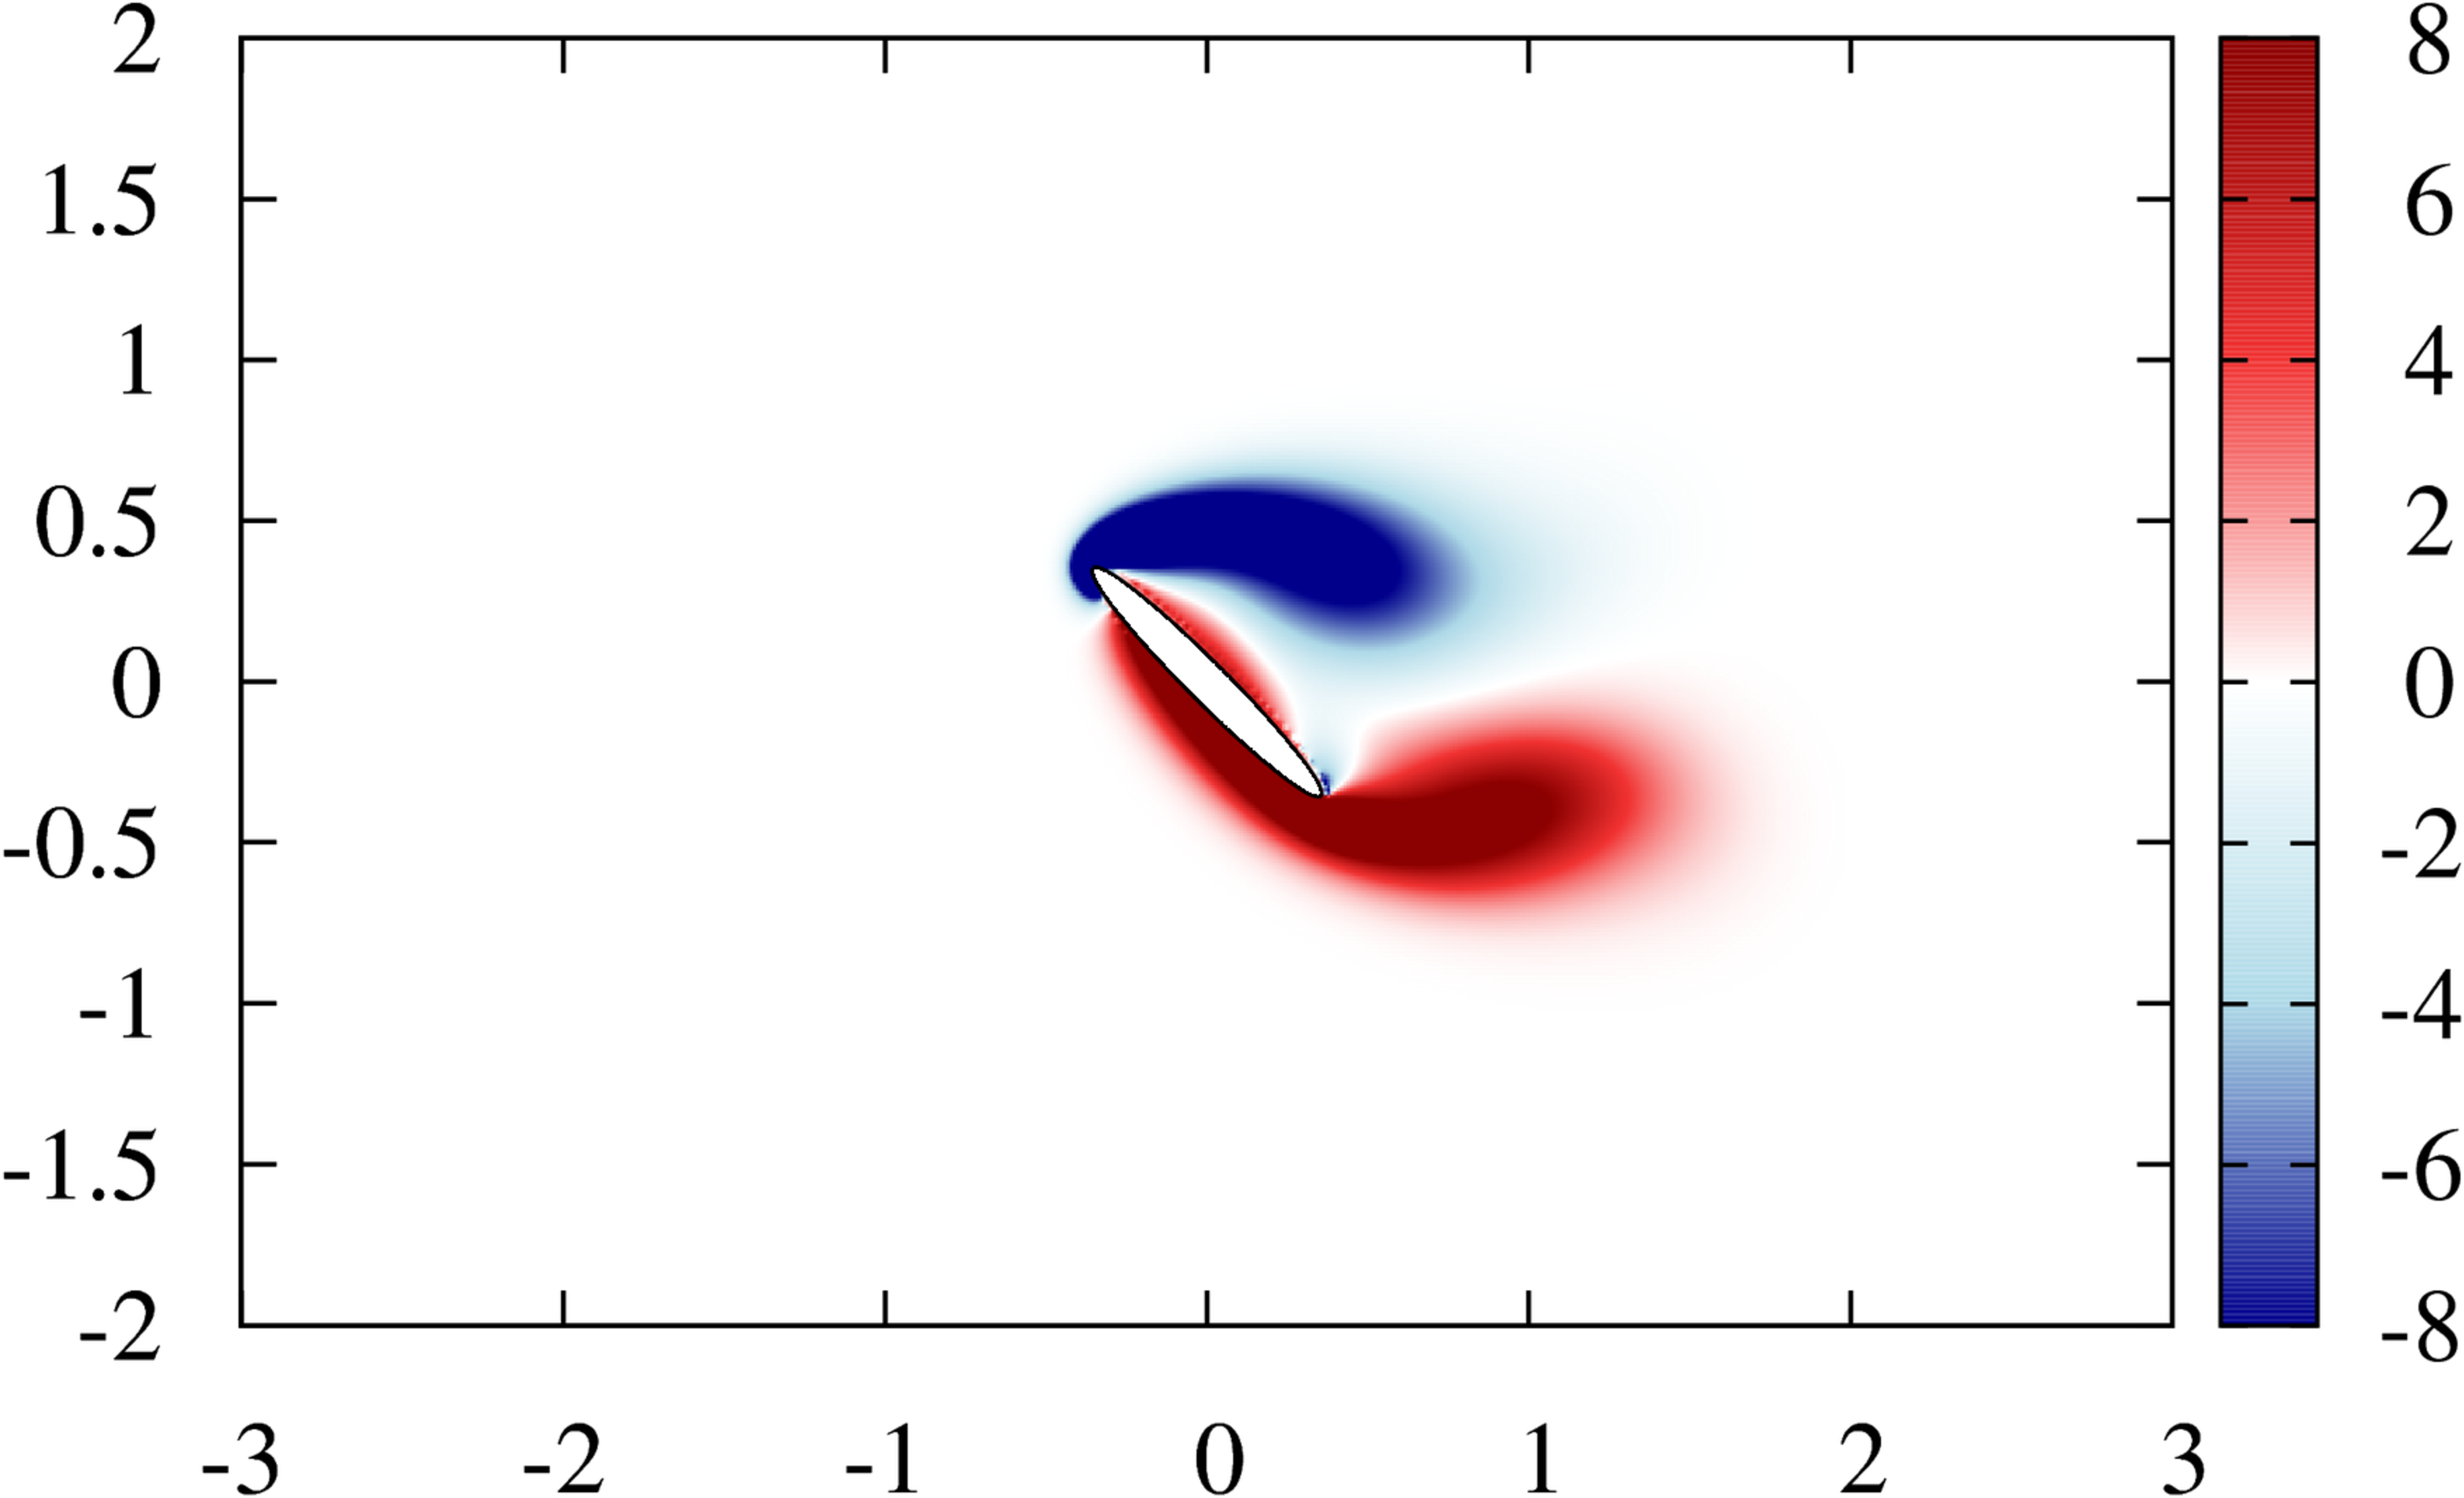
\includegraphics[width=0.4\textwidth]{figs/flap1000.pdf} \\
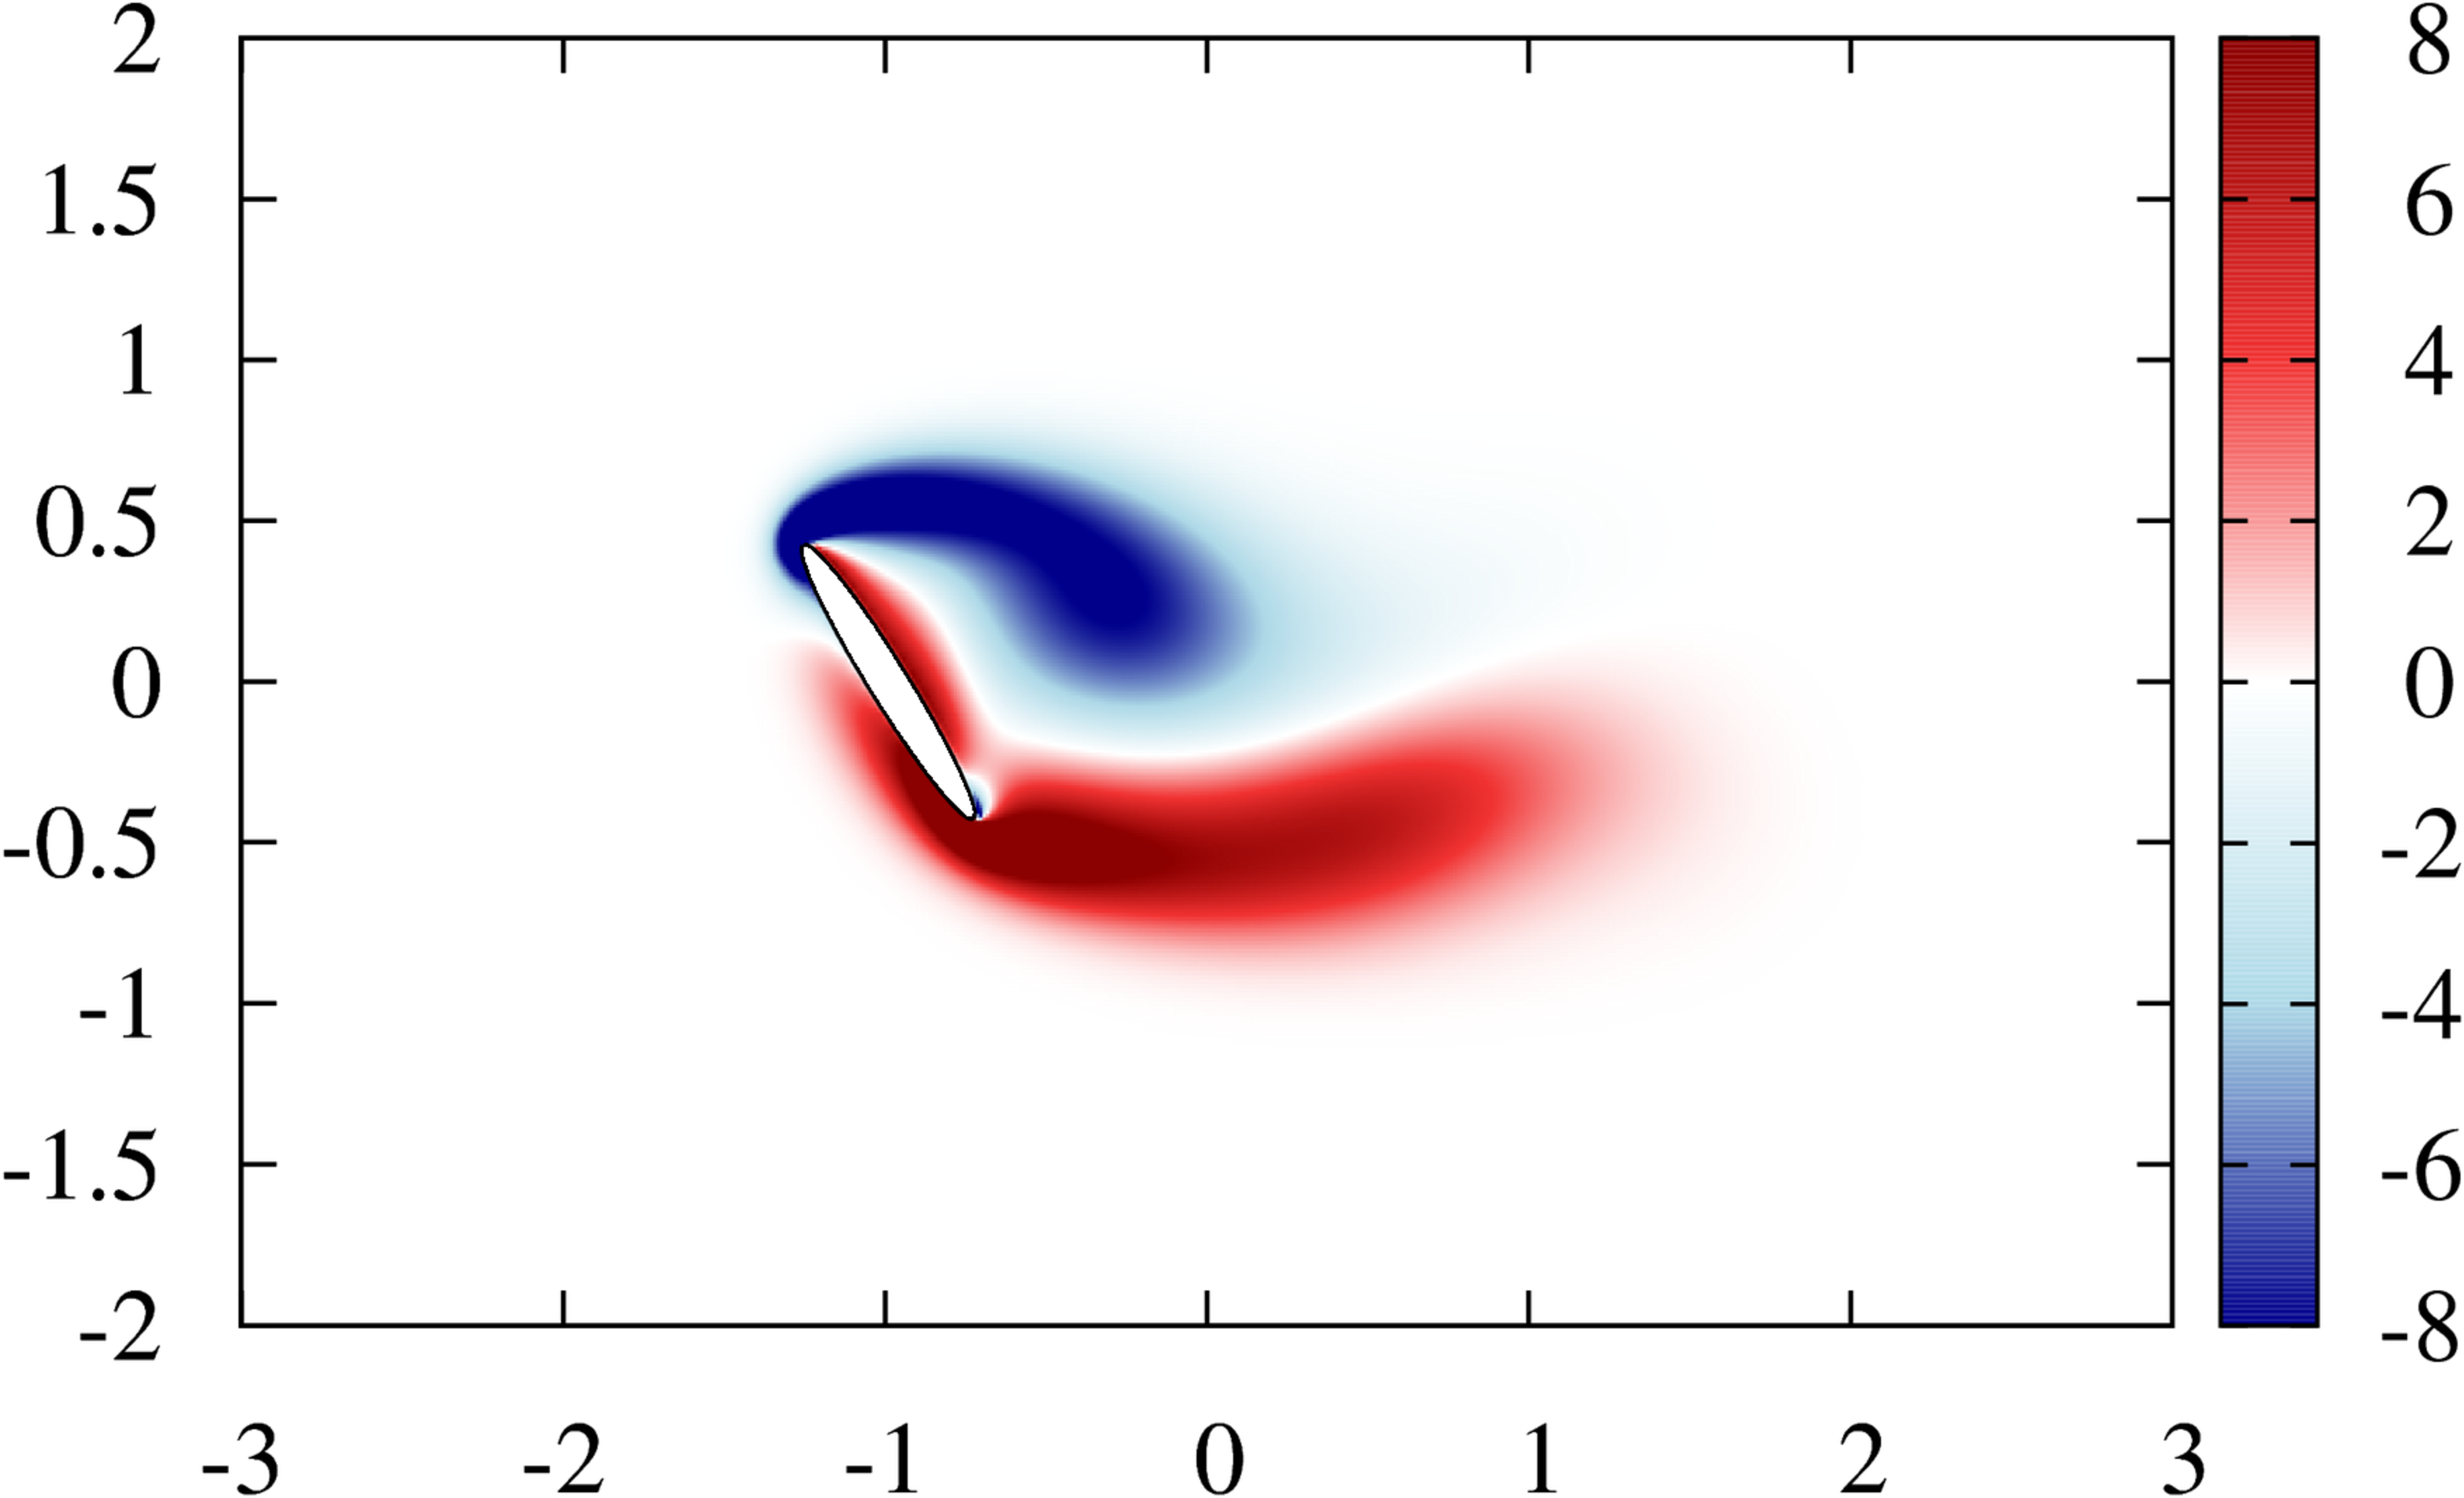
\includegraphics[width=0.4\textwidth]{figs/flap1500.pdf} &
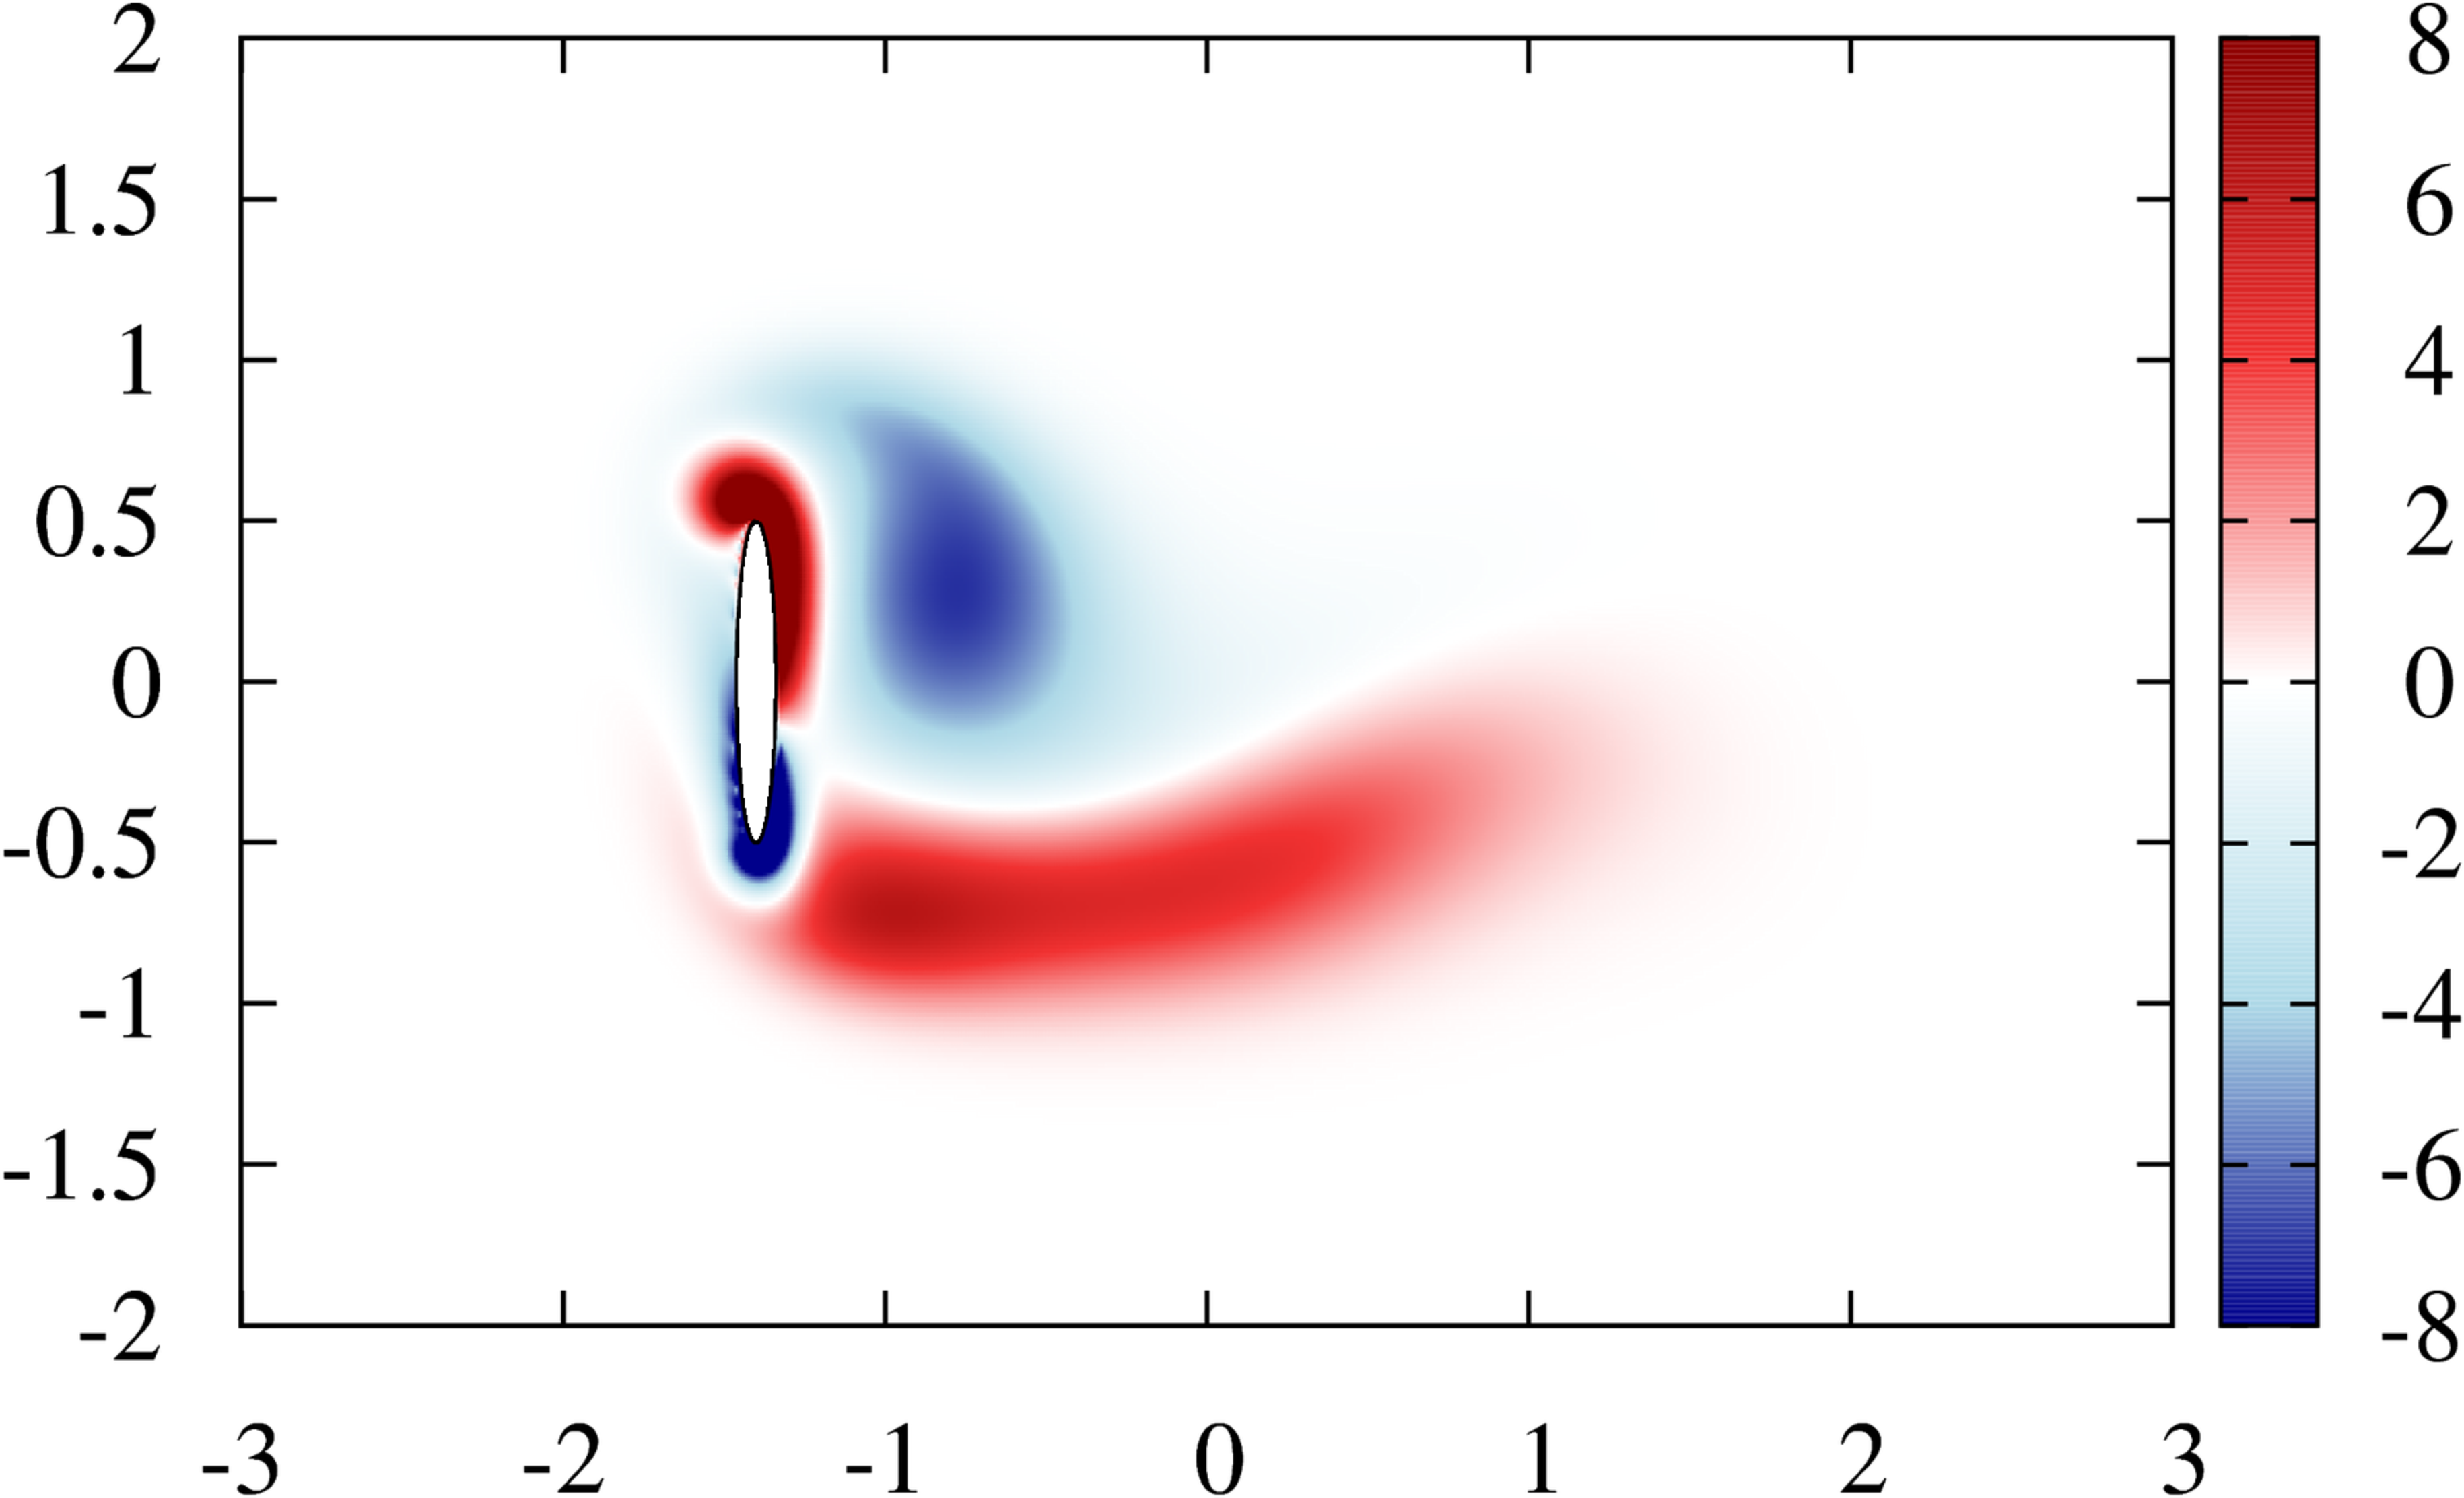
\includegraphics[width=0.4\textwidth]{figs/flap2000.pdf} \\
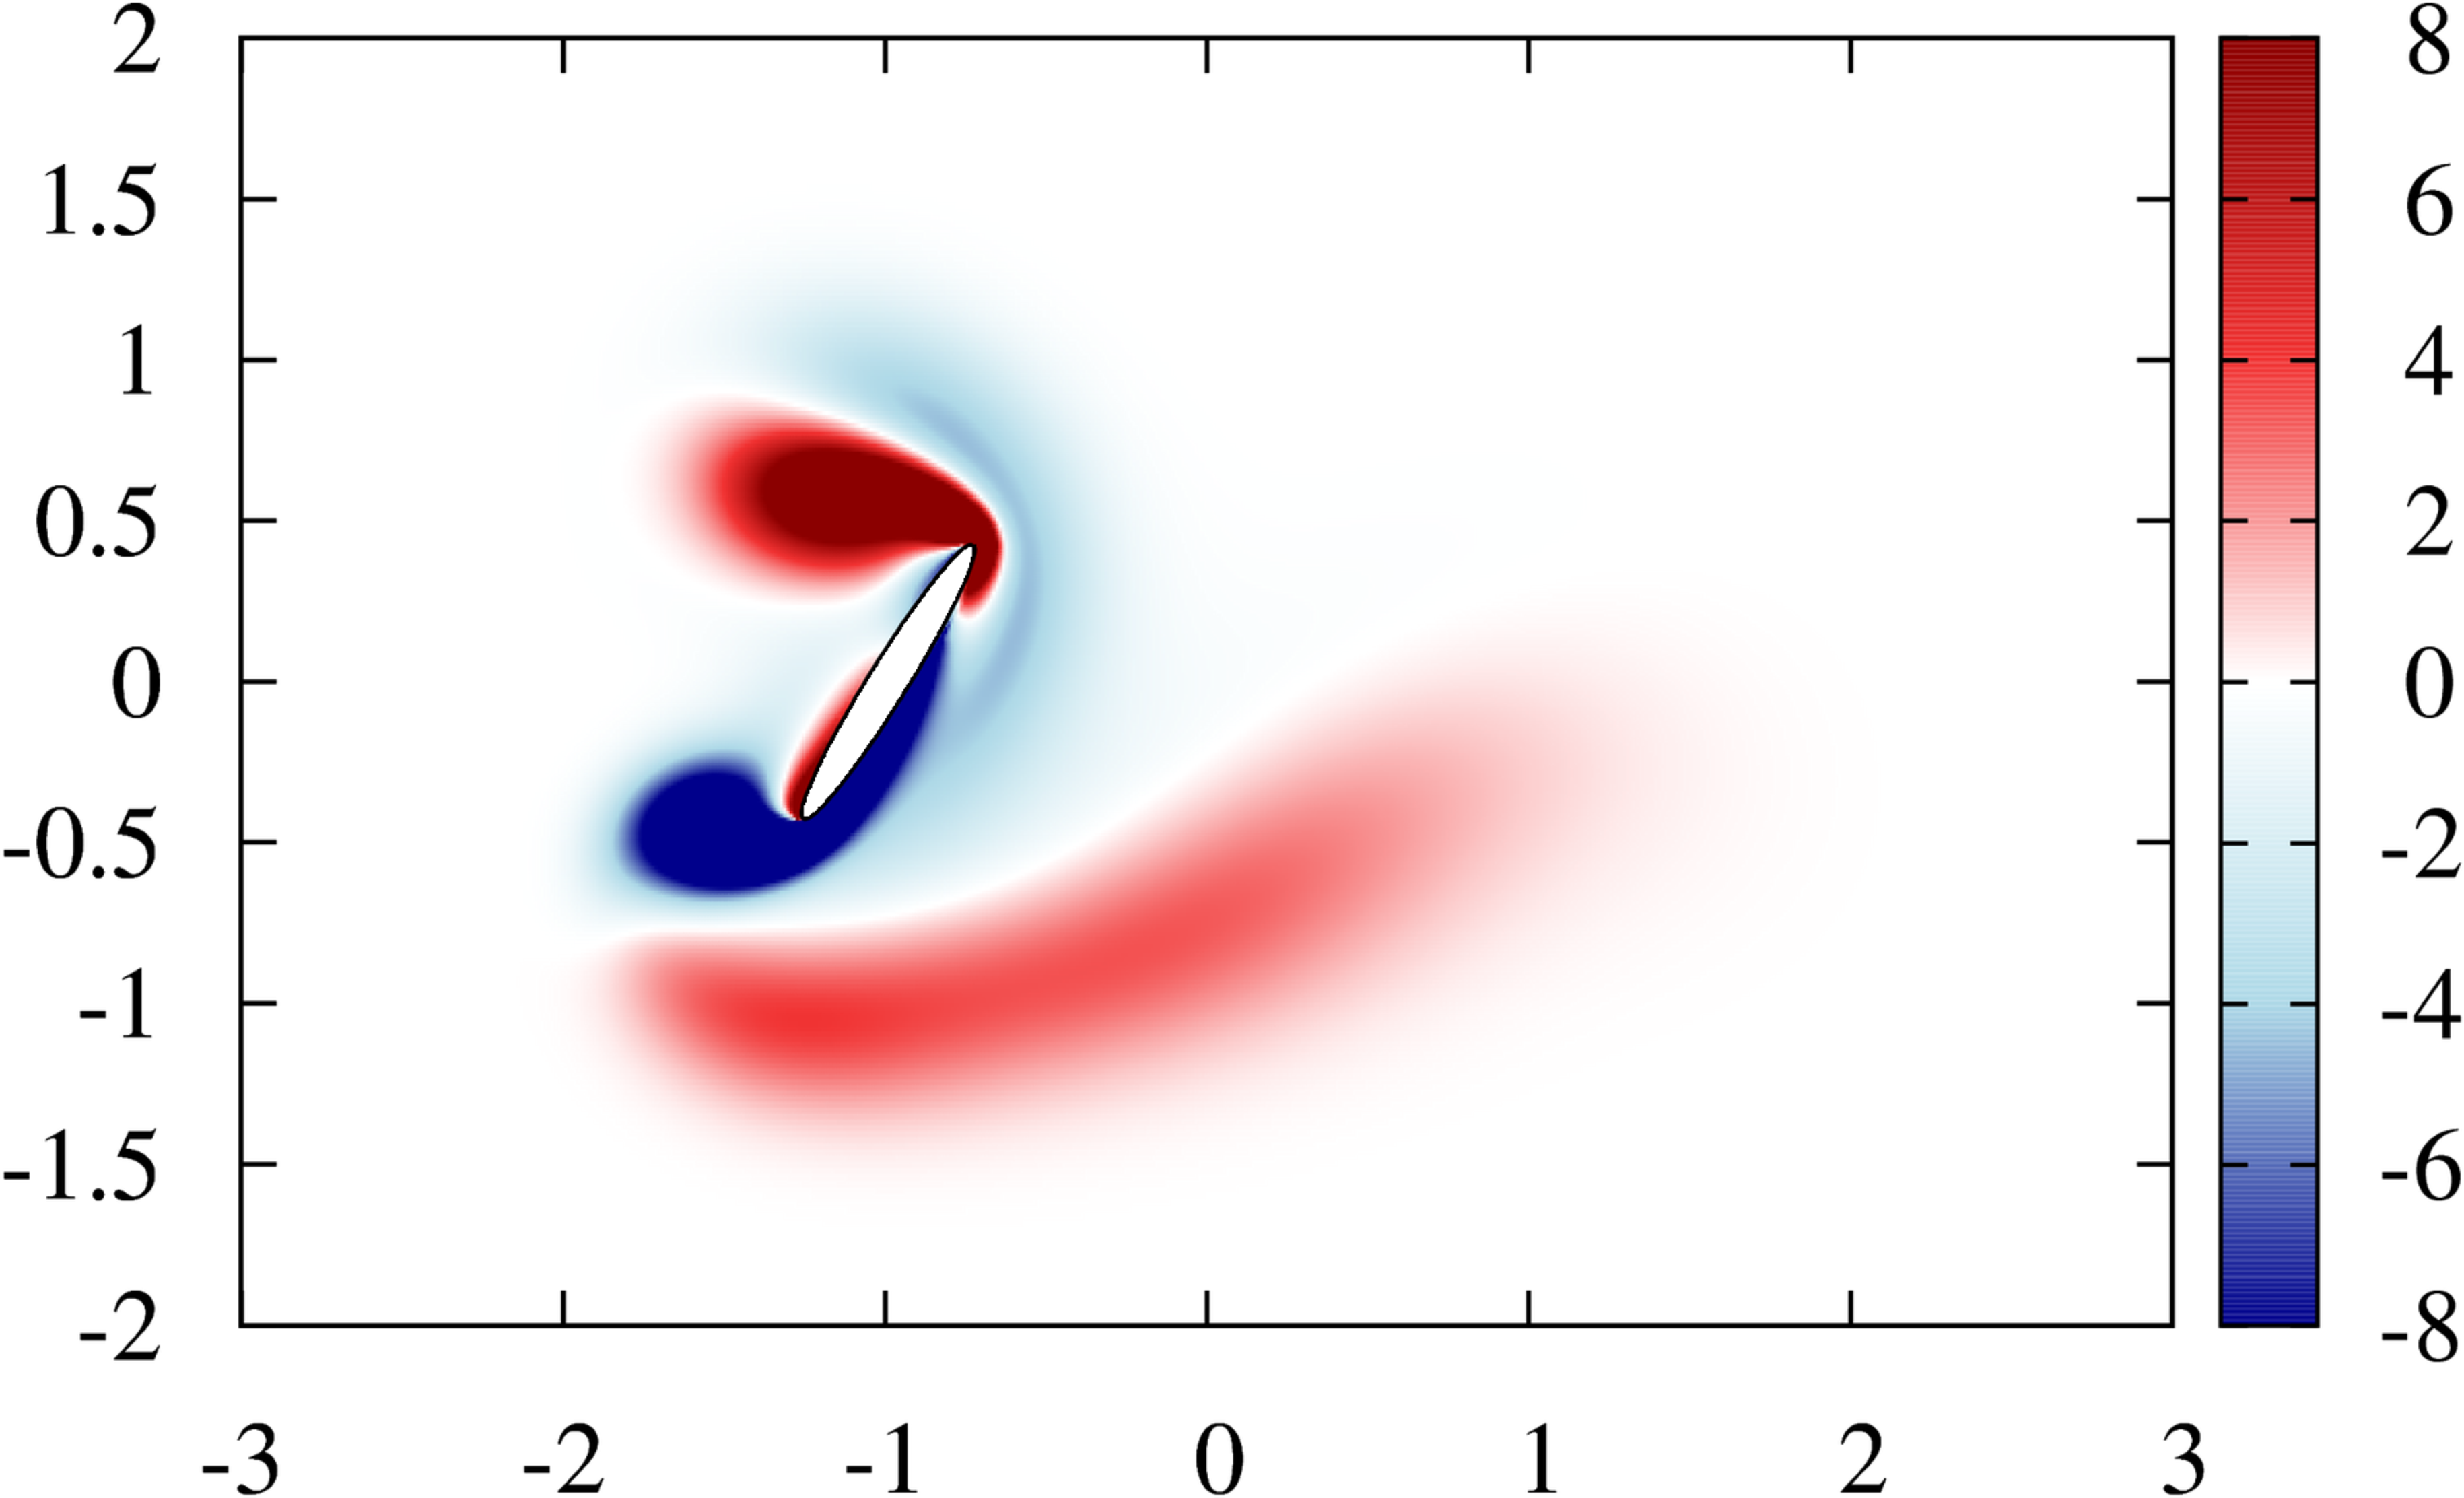
\includegraphics[width=0.4\textwidth]{figs/flap2500.pdf} &
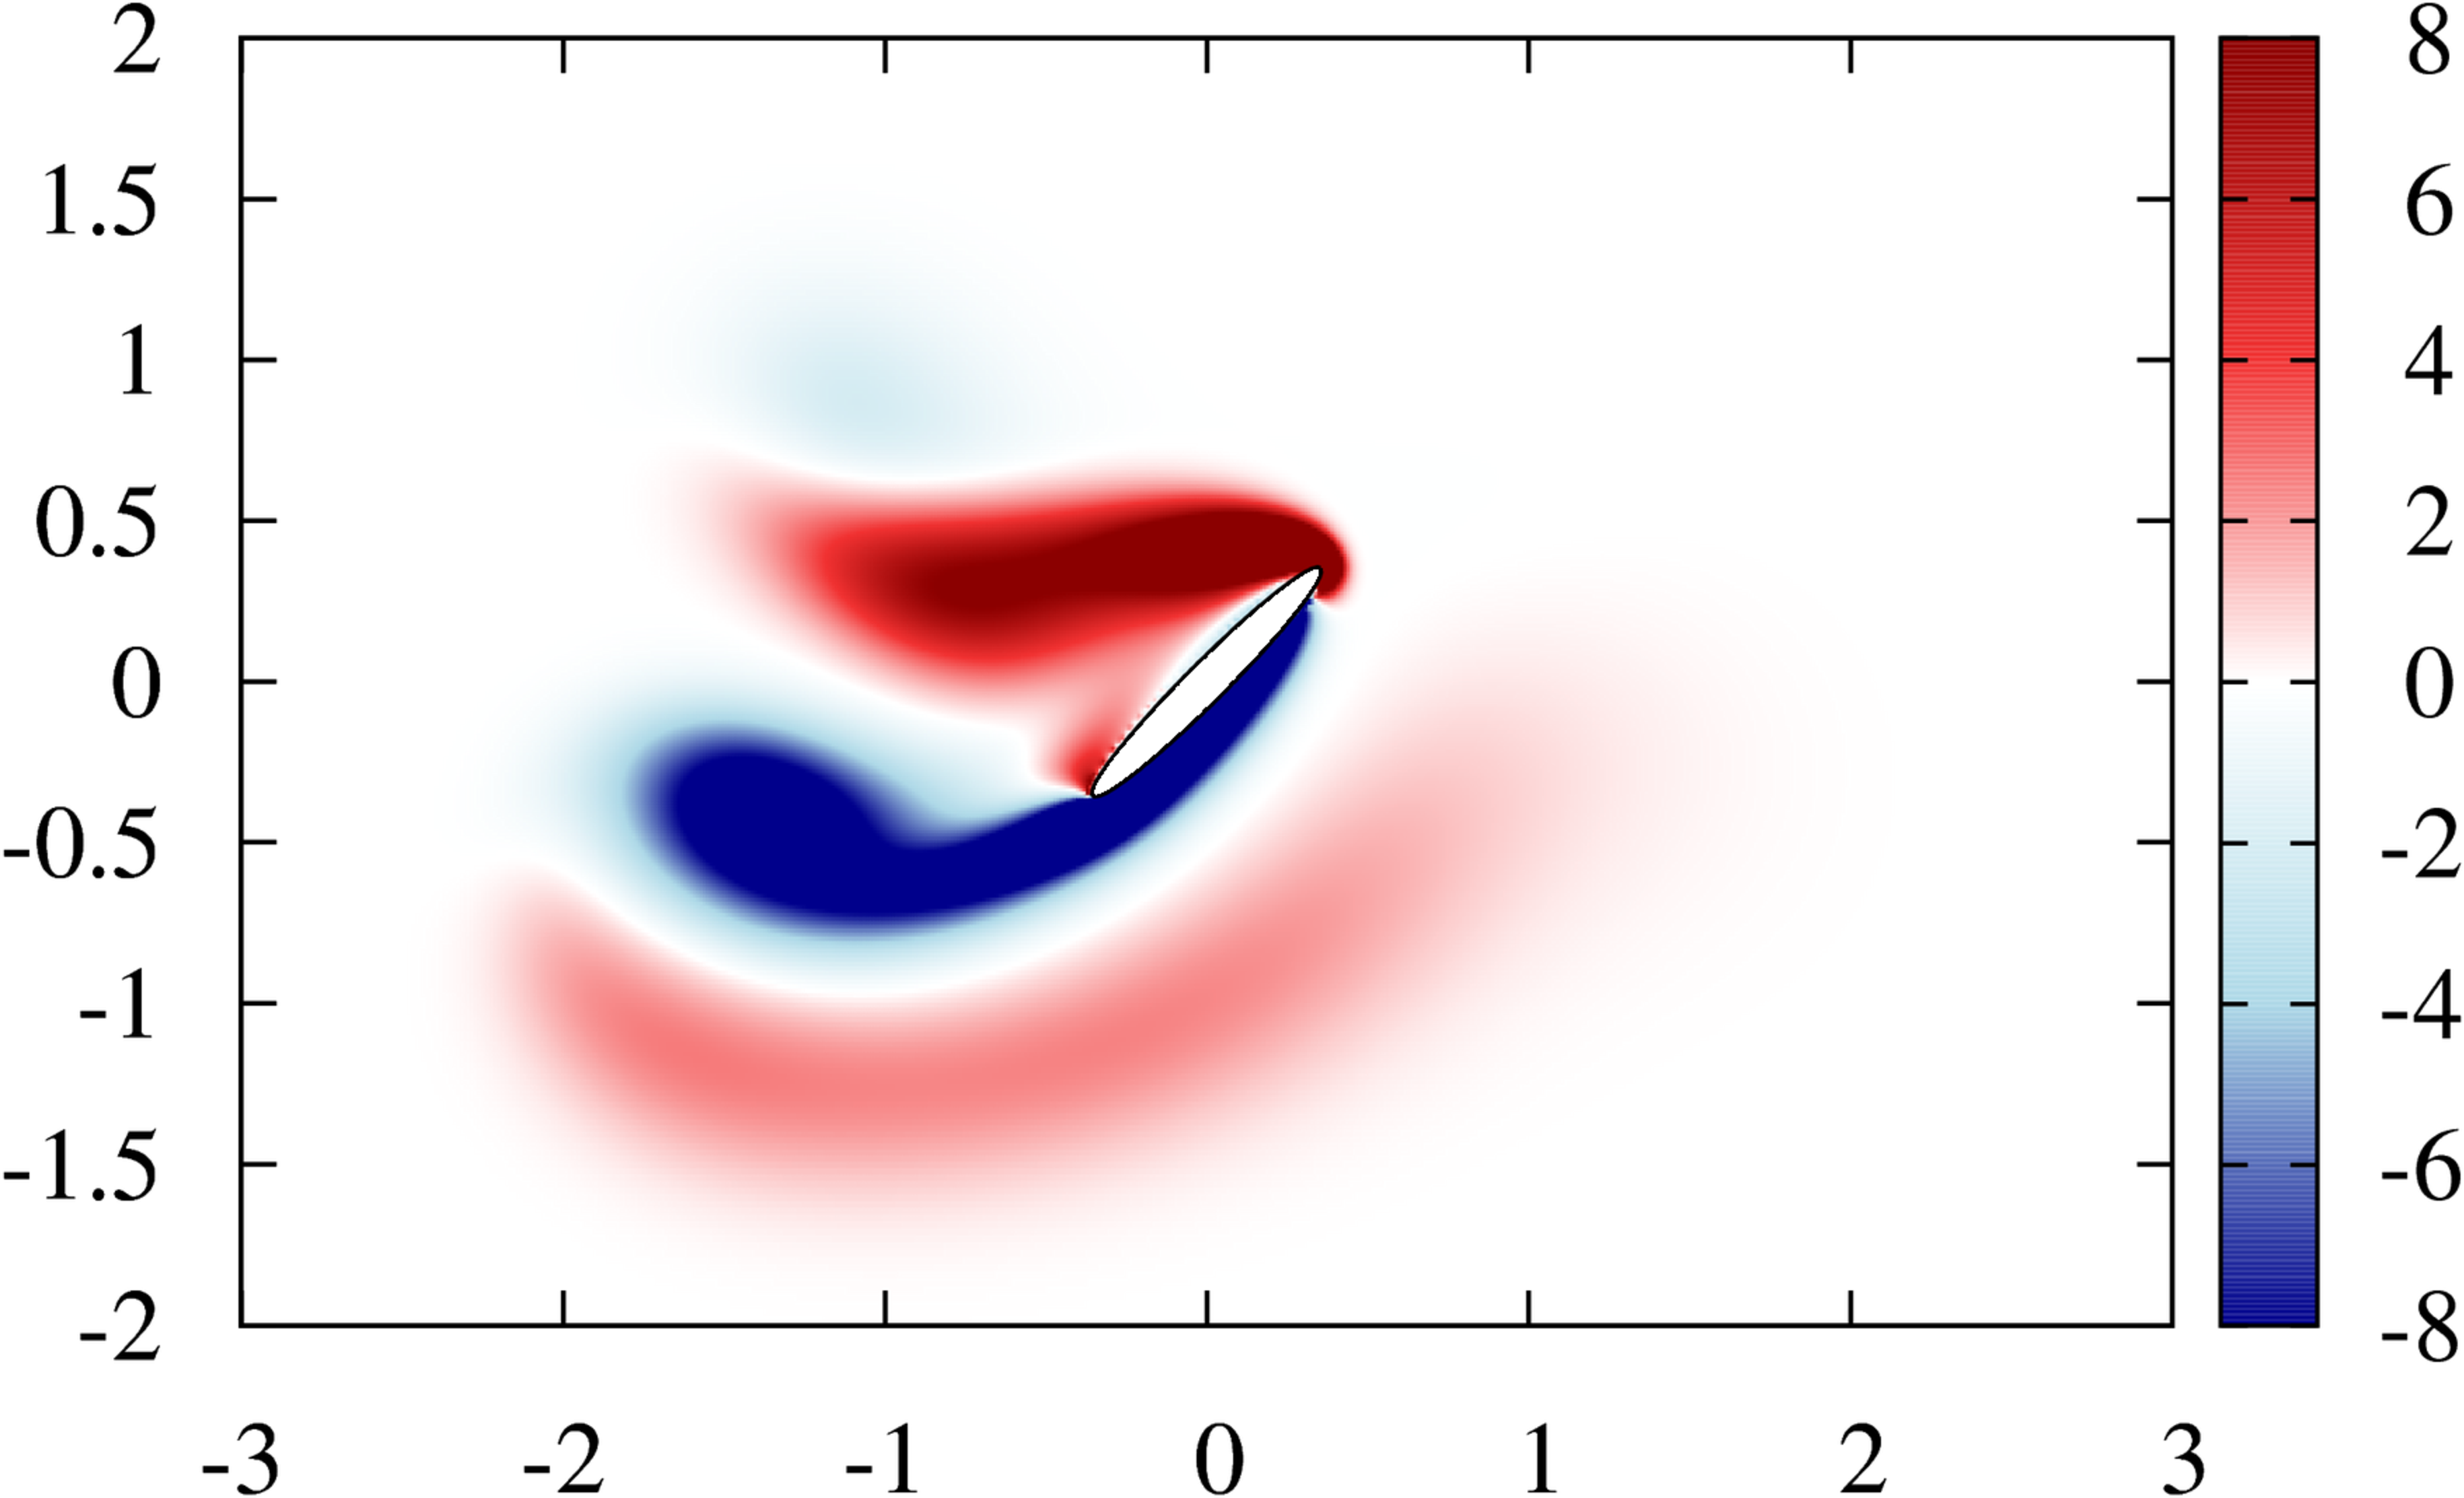
\includegraphics[width=0.4\textwidth]{figs/flap3000.pdf} \\
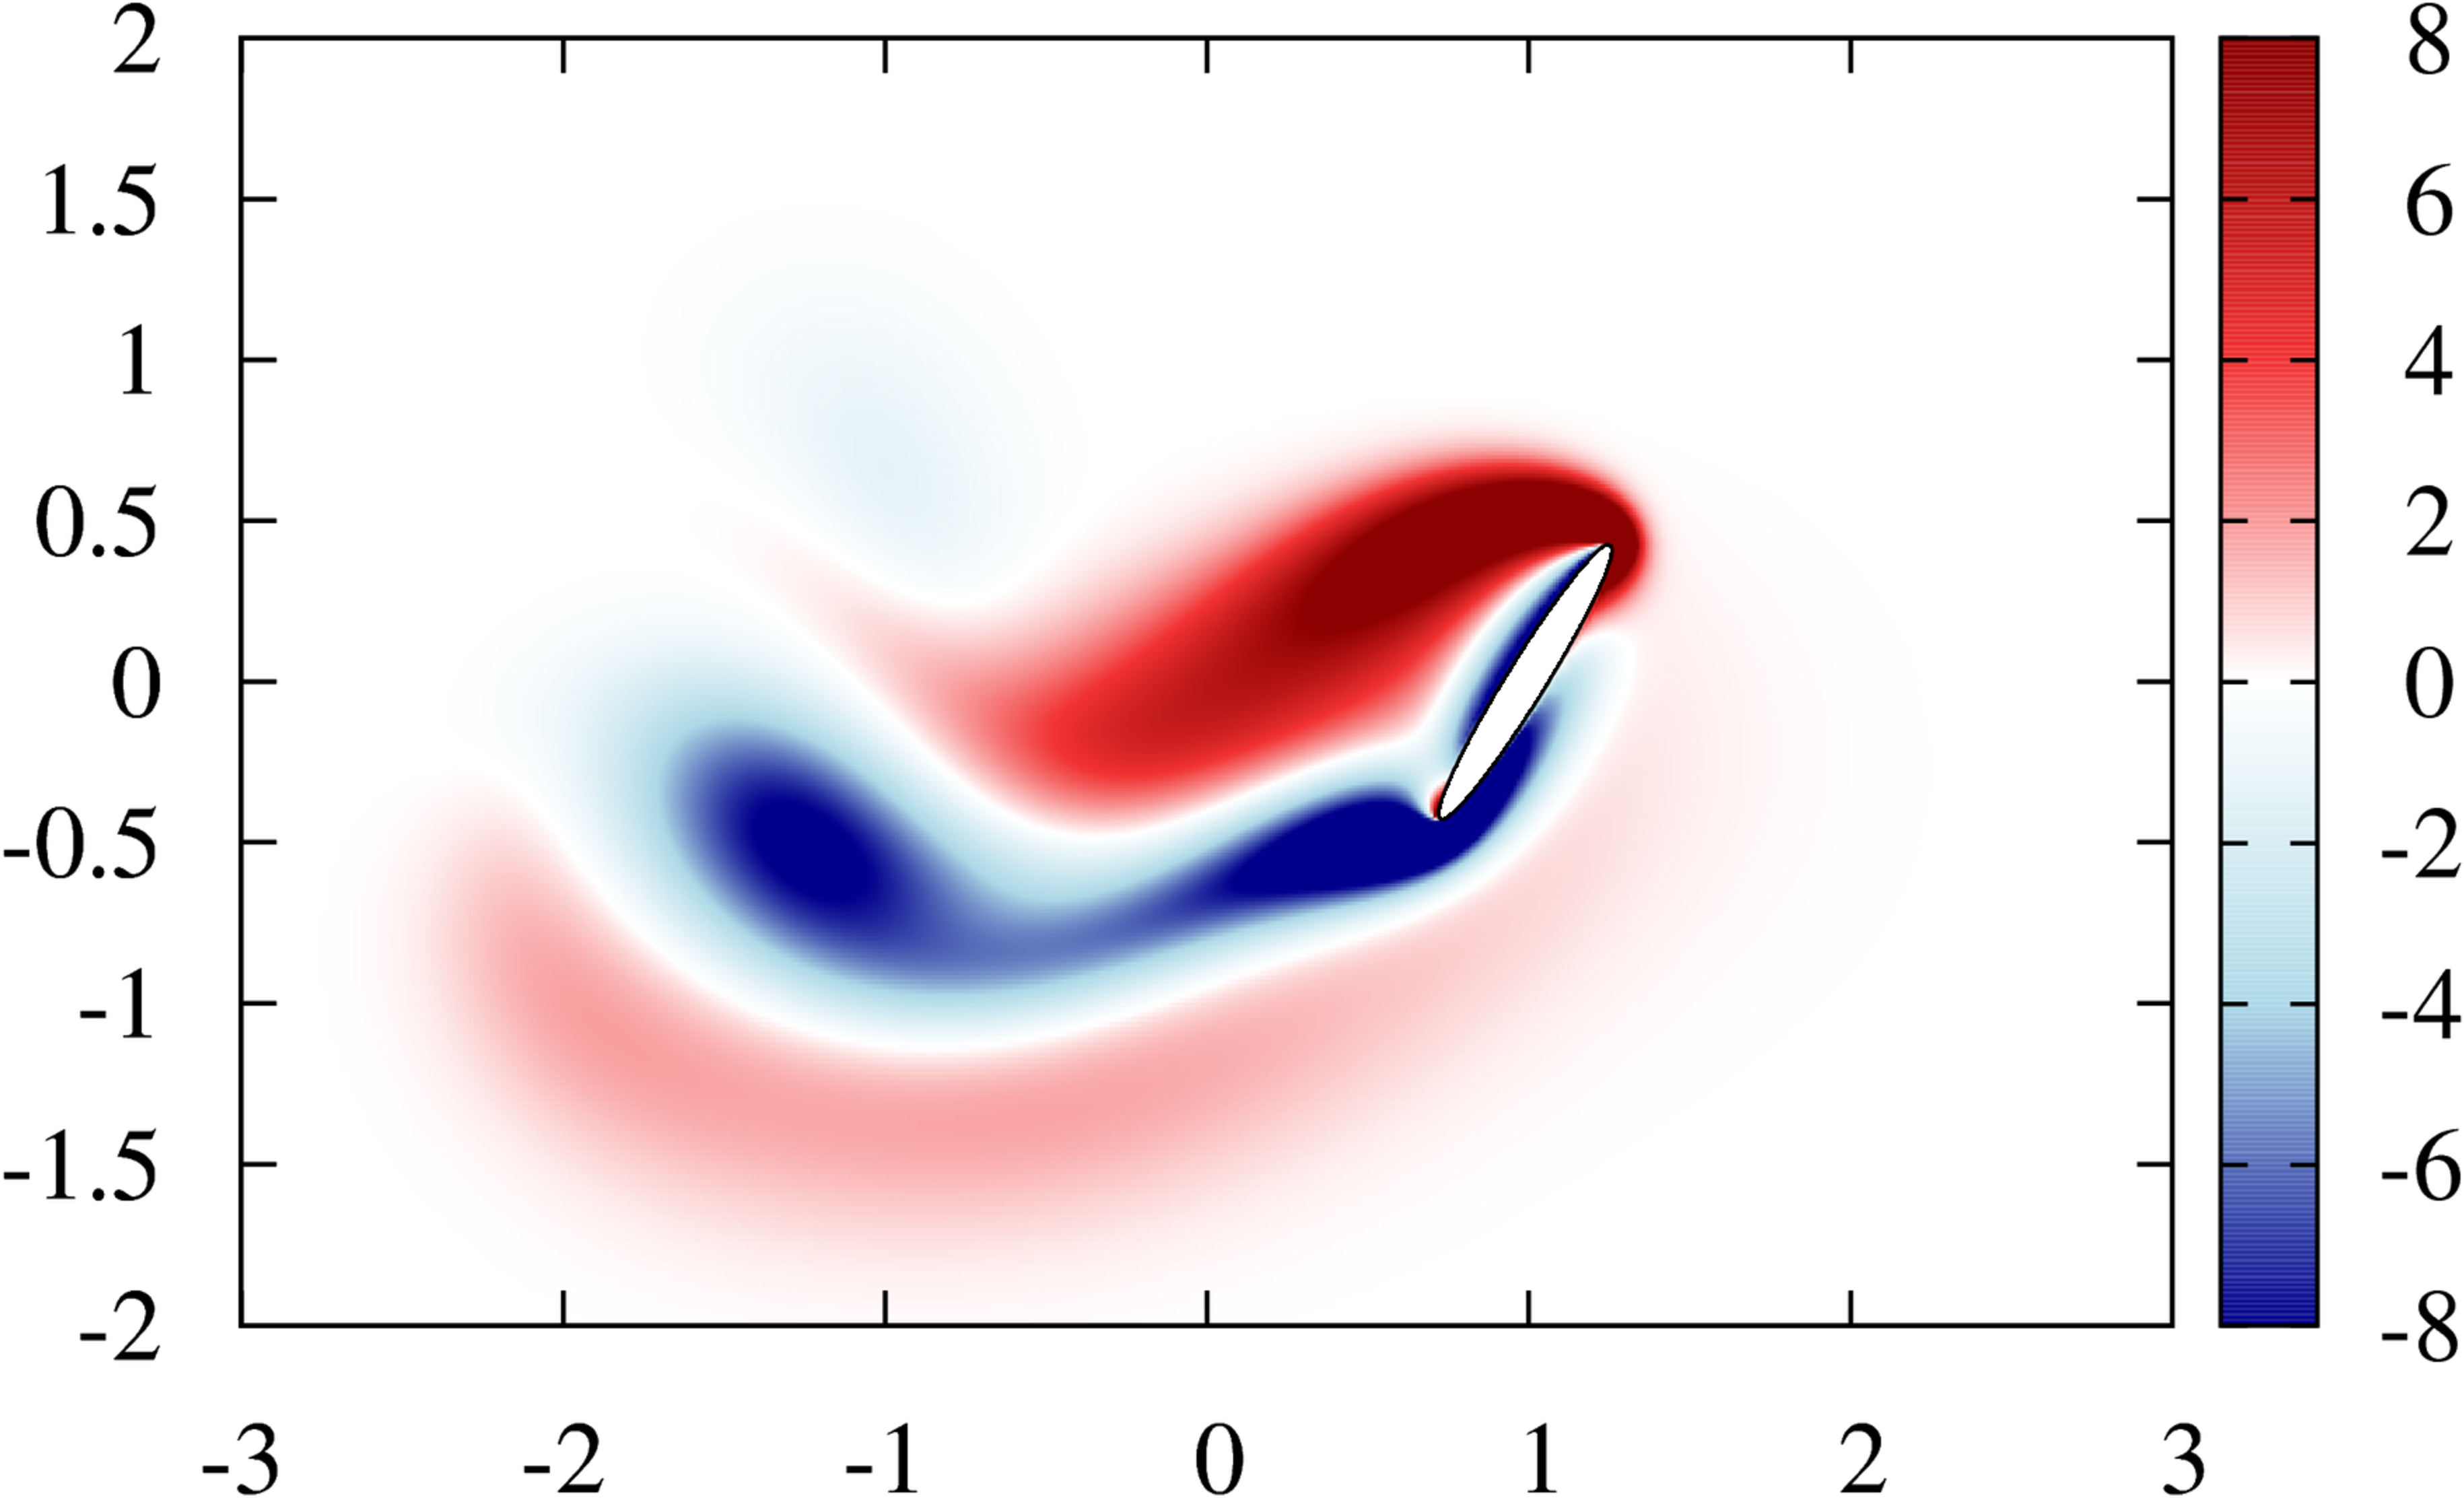
\includegraphics[width=0.4\textwidth]{figs/flap3500.pdf} &
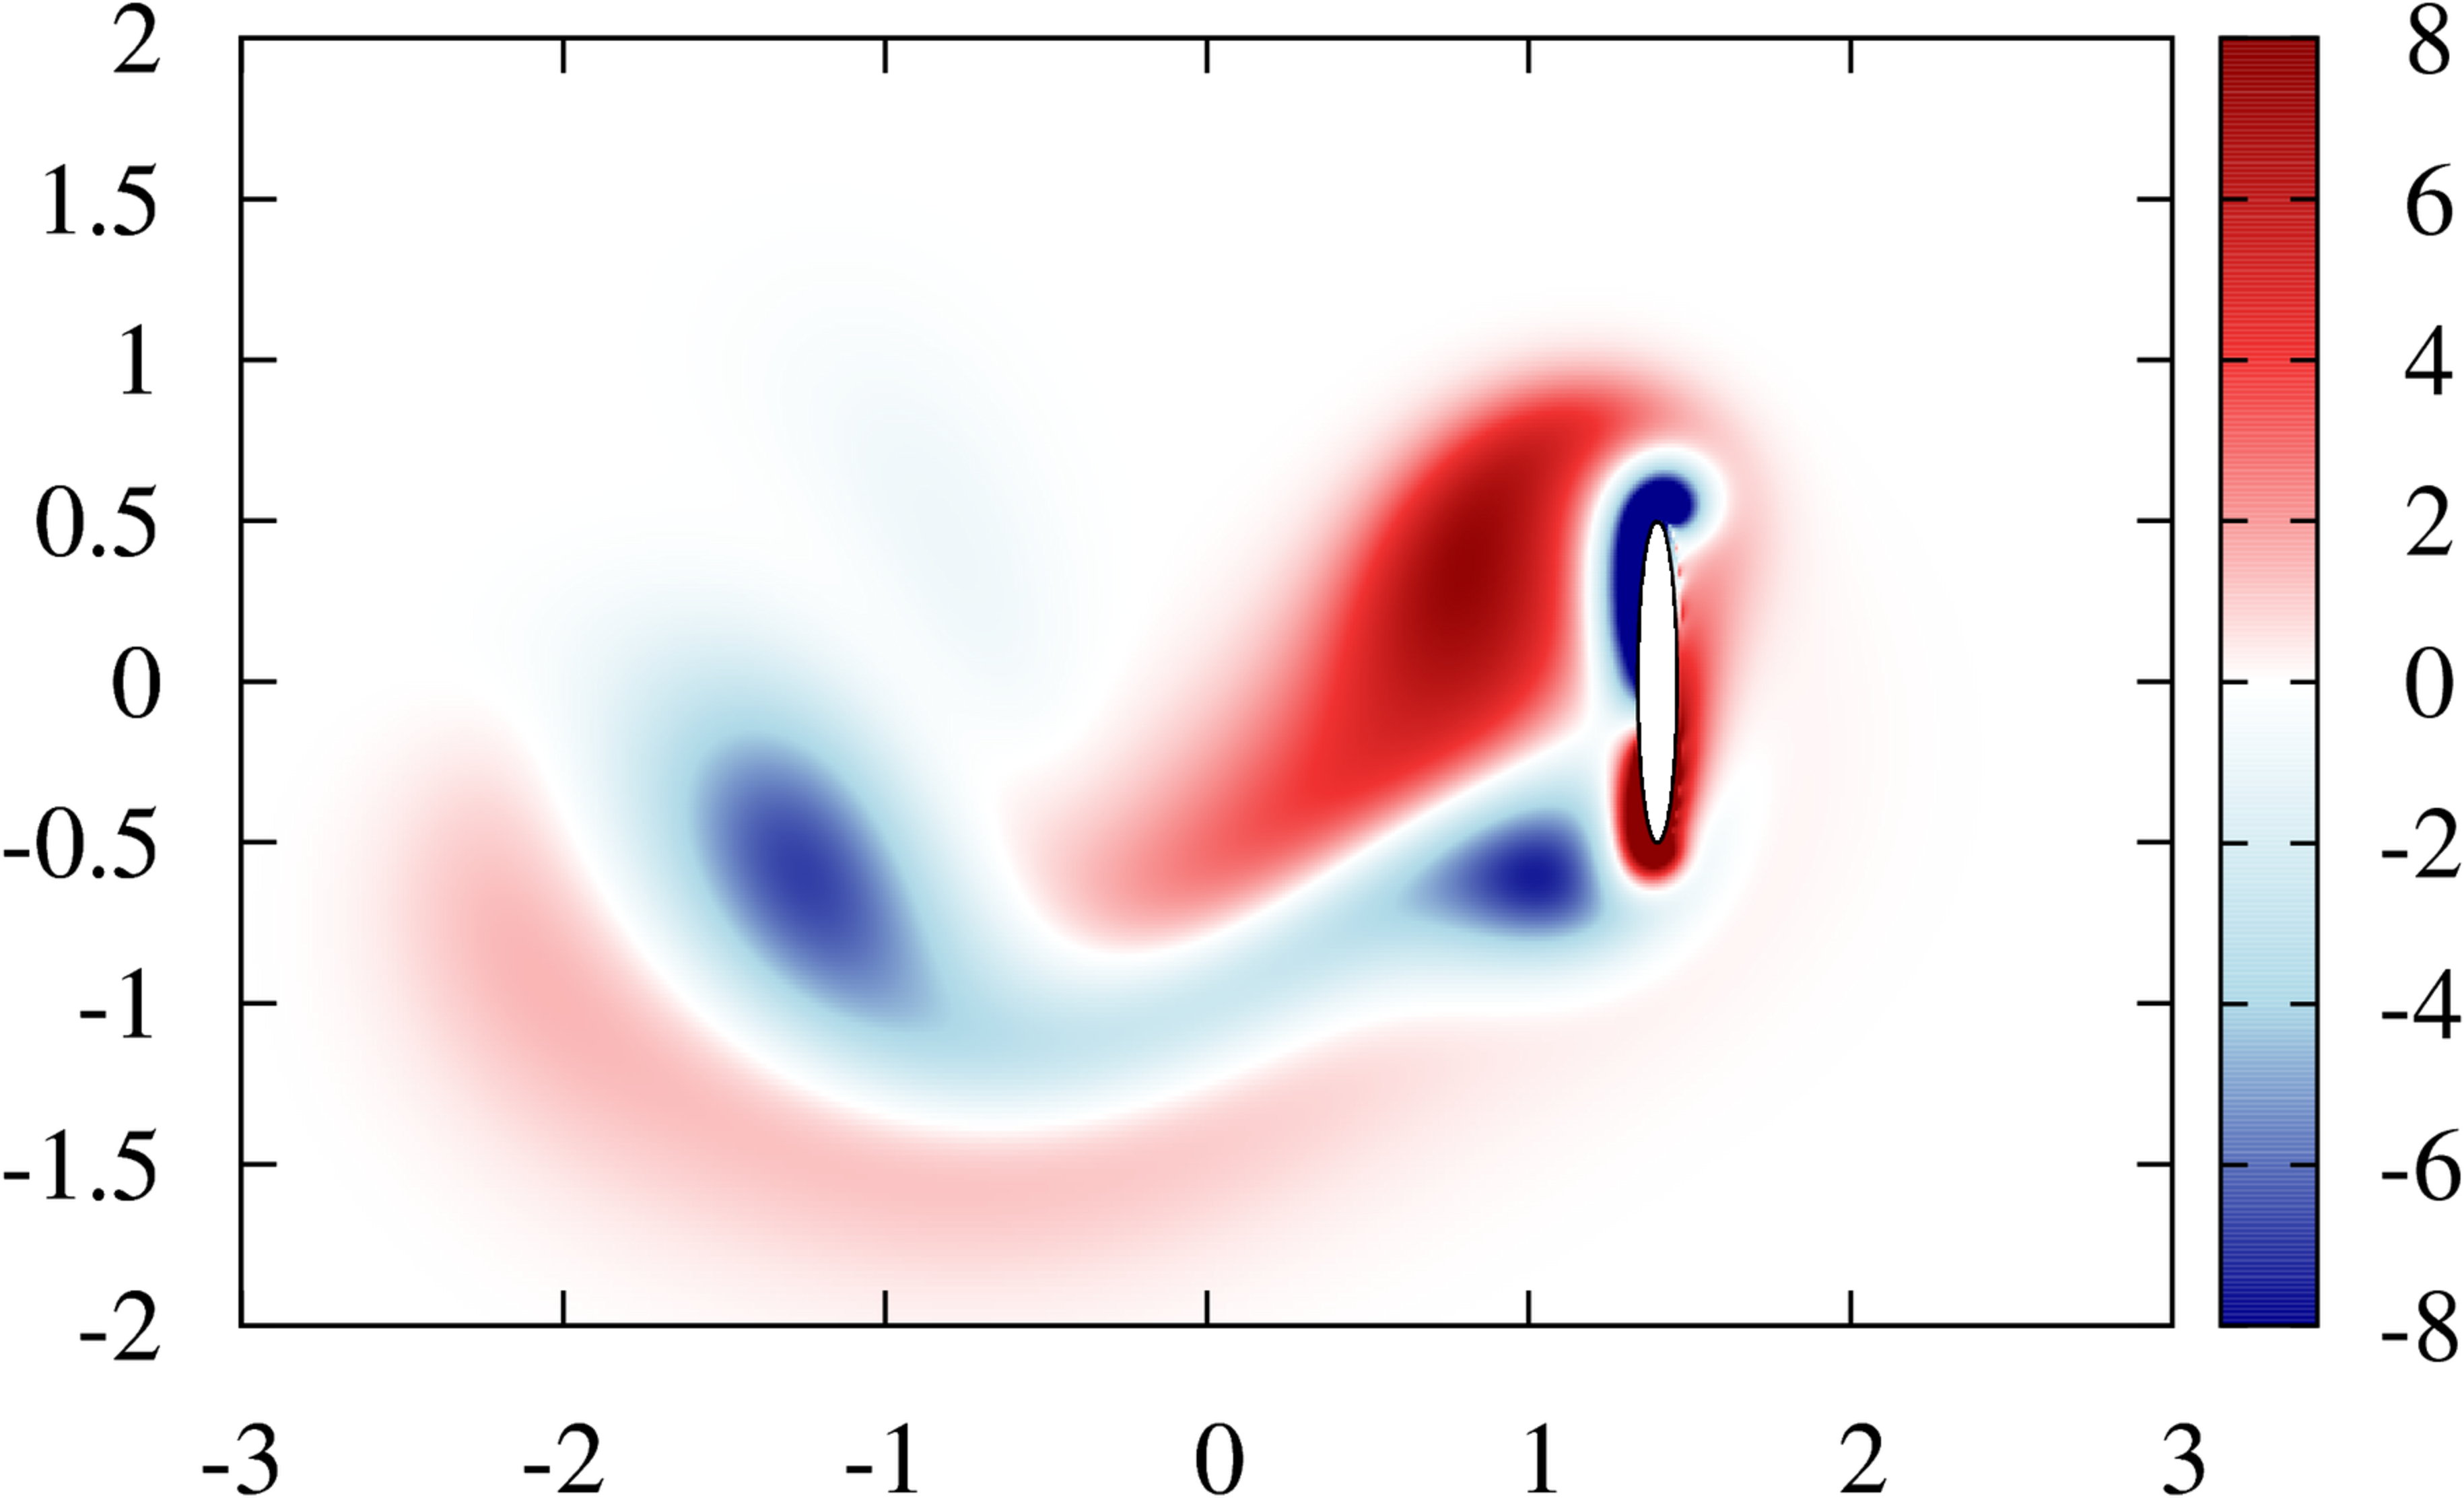
\includegraphics[width=0.4\textwidth]{figs/flap4000.pdf}
\end{array}$
\caption{Vorticity field of the flow around a flapping airfoil at equally spaced time instants in the first cycle of flapping: {$T=0.125$, $0.25$, $0.375$, \ldots}.}
\label{fig:flapping}
\end{figure*}


\section{Implementation details}


The various formulations of the {\ibm} that have been published in the open literature can all be written in a form similar to Equation \eqref{eq:newsystem}. We view this form as a general framework to implement a variety of fluid solvers. If there is no immersed body, then the matrices $E$ and $E^T$ are zero and the system solves the unmodified Navier-Stokes equations. In another \ibm technique, known as the direct-forcing method,\cite{Fadlun2000} the $E$ matrix is again absent, while the matrix $A$ can be appropriately modified so that the no-slip condition is enforced at the boundary locations that intersect with the grid. In this way, we build the \cuibm framework to allow the testing of different solvers and the development of new ones.

The code is written in \texttt{C++} and uses \gpu\ hardware via \cuda. It consists of a base class, \texttt{NavierStokesSolver}, which stores all the matrices required for the solution of the Navier-Stokes equations in a rectangular domain without immersed bodies. The class \texttt{NSWithBody} inherits from this class and also stores the information regarding any bodies present in the flow domain. The different {\ibm} solvers such as \texttt{TairaColoniusSolver} and  \texttt{FadlunEtAlSolver} inherit from this class. Each derived class makes use of the body information and has its own version of the methods used to generate the sub-matrices $A$ and $Q$, specific to the solver used.

The flow description and the simulation parameters are supplied to the code using input files. There are four input files:
\begin{itemize}
\item[$\triangleright$] Flow file: Specifies the velocity boundary conditions on the domain and the kinematic viscosity of the fluid.
\item[$\triangleright$] Domain file: Provides information regarding the grid and flow domain. Currently, only Cartesian grids are supported but the mesh can be stretched exponentially whenever required.
\item[$\triangleright$] Body file: Specifies the locations of the boundary points and the rigid-body motion that the body undergoes during the simulation.
\item[$\triangleright$] Simulation file: Contains the numerical parameters relevant for the simulation, such as the time step, {\ibm} schemes, time-stepping schemes, etc.
\end{itemize}

The various time-stepping schemes available are explicit Euler, second-order Adams-Bashforth and third-order Runge-Kutta methods for the convection terms, and explicit Euler, implicit Euler, second-order Adams-Bashforth and Crank-Nicolson schemes for the diffusion terms. All spatial discretizations have been evaluated using central differences.

The matrices and linear systems in \cuibm are stored and solved using the {\cusp} library,\cite{Cusp}  distributed freely by the {\nvidia} Corporation under the Apache License. 
 This library provides storage formats and routines for sparse linear algebra and has been optimized to run on {\nvidia} {\gpu}s when compiled using the \texttt{nvcc} compiler. The same code can also be compiled to run on {\cpu}s, when it makes use of the Math Kernel Library from Intel. The entire code is written using the {\thrust} library, now shipping with the {\cuda} compiler, which consists of a number of basic algorithms that are {\gpu}-optimized versions of those in the \texttt{C++} Standard Template Library. These functions are templated over the memory type, and the same code can be compiled to run on both {\cpu}s and {\gpu}s.

We use \textsc{yaml}\cite{YAML2009} to parse the human-readable input files. This code is distributed under the MIT license and we have included parts of it in our code base.

The {\cusp} library provides various pre-conditioners and solvers, and all sparse linear algebra in \cuibm is performed using {\cusp}.  Several custom {\cuda} kernels were written so that all operations take place on the {\gpu} and the data transfer between the host and the device is minimized. It is well known that sparse matrix computations are memory-bound, and the larger memory bandwidth provided by {\gpu}s result in a speed-up compared to the code running on a {\cpu}. However, we have not implemented an optimized \cpu\ code and thus are not able to report comparative performance metrics.


\newthought{We release} the {\cuibm} code under the MIT License, and maintain a Bitbucket repository at \href{https://bitbucket.org/anushk/cuibm/}{https://bitbucket.org/anushk/cuibm/}.

\noindent We also provide \textsc{matlab} and \texttt{Gnuplot} postprocessing scripts to plot the various flow variables. User documentation is currently being written.

\bibliography{ibm,cfd,vortexflow,scicomp,biolocomotion}
\bibliographystyle{plainnat}



\end{document}
